% !TEX root = mythesis.tex

%==============================================================================
\chapter{Spectrum of Excitons}
\label{sec:excitons}
%==============================================================================
In this chapter, we will discuss the algorithm that was created and used to find the correlation functions, and finally the results for the binding energy of the particle-hole pair. We will discuss what is potentially the physical meaning behind the results, we have obtained.

\section{Data Generating}

The data gathering is done by the use of an algorithm which was developed specifically for calculating the one-body and two-body correlation functions. It can be easily customized for the generation of one- and two-particle correlators with different set of creation and annihilation operators.

The algorithm takes as an input a set of momenta and $\phi$ fields. The latter are generated independently using the HMC method of sampling. The reasons for this separation is due to the computational cost of generating these fields, to be able to cross-check the results by using the same values, and for multiple uses for calculating other observables. After the input, the program computes the operators which construct the correlation functions for all possible combinations of momenta ($k$) and bands labels ($\sigma$), both at the source ($t=0$) and at the sink ($t=\tau$), as well as for particles and holes
\begin{equation}
    \mathcal{O}[\pm\phi] = {\psi^{k\sigma_{sink}}_{y}}^{*}M^{-1}_{\tau,y;0,x}[\pm\phi]\psi^{q\sigma_{scr}}_{x} = M^{-1}_{k\sigma_{sink};q\sigma_{scr}}[\pm\phi].
\end{equation}
This is done by computing a propagator from the source ($M^{-1}_{\tau,y;0,x}\psi^{q\sigma_{scr}}_{x}$) using FGMRES and then multiplying it with the sink. After the "pool" of all fermionic operators is completed, the code applies the physics constraints on the whole data set which tells how to draw the correlation functions from it. In the one-body case the constraint is the momentum conservation at the source and sink, meaning the momenta should be equal ($k=q$). In the two-body case, we have two kinds of correlators. The particle-hole pair correlation function $\langle phh^\dagger p^\dagger\rangle$ and the particle-particle pair $\langle ppp^\dagger p^\dagger\rangle$. The first can be extracted by giving again constraint on the momentum at the source and at the sink; not on the individual momenta but on the total momentum, resulting in a lot more different combination of indices and labels. The other correlator that we want to extract, is more difficult to do so, because not only we have to apply the total momentum conservation but to take into account the additional Wick contractions. The basic flowchart of the algorithm is shown on \cref{fig:alg_flow}.
\begin{figure}[!htbp]
    \begin{center}
      % \scalebox{0.66}{
      \scalebox{1.0}{
        \begin{tikzpicture}[node distance=1.9cm]
            \tikzstyle{startstop} = [rectangle, rounded corners, minimum width=3cm, minimum height=1cm,text centered, draw=black, fill=red!30]
            \tikzstyle{io} = [trapezium, trapezium left angle=70, trapezium right angle=110, minimum width=3cm, minimum height=1cm, text centered, draw=black, fill=blue!30]
            \tikzstyle{process} = [rectangle, minimum width=3.5cm, minimum height=1cm, text centered, text width=3cm, draw=black, fill=orange!30]
            \tikzstyle{decision} = [diamond, minimum width=3cm, minimum height=1cm, text centered, text width=3cm, draw=black, fill=green!30]
            \tikzstyle{arrow} = [thick,->,>=stealth]

            \node (start) [startstop] {Start};
            \node (in1) [io, below of=start] {Input the $\phi$ fields};
            \node (pro1) [process, below of=in1] {Calculate $\mathcal{O}_i[\phi]$};
            \node (dec1) [decision, below of=pro1, yshift=-1.5cm] {One- or Two-body correlator};
                \node (dec1a) [decision, left of=dec1, xshift=-3cm] {$k=q$};
                    \node (pro1a1) [process, below of=dec1a, yshift=-1.5cm] {Ensemble average};
                    \node (pro1a2) [process, below of=pro1a1] {$C_k(\tau)$};
                \node (dec1b) [decision, right of=dec1, xshift=3cm] {$P_{sink} = P_{scr}$};
                    \node (pro1b1) [process, below of=dec1b, yshift=-1.5cm] {$\left(\mathcal{O}_i[\phi]\mathcal{O}_j[\phi]\right)_{Wick}$};
                    \node (pro1b2) [process, below of=pro1b1] {Ensemble average};
                    \node (pro1b3) [process, below of=pro1b2] {$C_P(\tau)$};
            \node (out1) [io, below of=dec1, yshift=-7.5cm] {Output the correlators};
            \node (stop) [startstop, below of=out1] {Stop};

            \draw [arrow] (start) -- (in1);
            \draw [arrow] (in1) -- (pro1);
            \draw [arrow] (pro1) -- (dec1);
            \draw [arrow] (dec1) -- node[anchor=south] {One} (dec1a);
                \draw [arrow] (dec1a) -- (pro1a1);
                \draw [arrow] (pro1a1) -- (pro1a2);
            \draw [arrow] (dec1) -- node[anchor=south] {Two} (dec1b);
                \draw [arrow] (dec1b) -- (pro1b1);
                \draw [arrow] (pro1b1) -- (pro1b2);
                \draw [arrow] (pro1b2) -- (pro1b3);
            \draw [arrow] (pro1a2) |- (out1);
            \draw [arrow] (pro1b3) |- (out1);
            \draw [arrow] (out1) -- (stop);
        \end{tikzpicture}
      }
    \end{center}
    \caption{Flowchart of the algorithm that calculates the one- and two-body correlation functions.}
    \label{fig:alg_flow}
\end{figure}

The raw output of the program is written into a different ASCII file for each combination of momenta configuration. Inside each file, the data is organized by configuration number. These files are then used as an input to a chain of scripts which handle the raw data. On every step of the data managing chain, a new HDF5 file is created, so that we can easily return to different set of groupings, check for bugs and errors, and it is less time-consuming when modifying the scripts or the data manually. The chain of scripts first organizes input into correlator groups with momenta subgroups, all collected in a HDF5 file encompassing the whole ensemble. After that, the scripts perform a bootstrap (see \cref{app:bootstrap}) on all correlation functions, and two new groups are created for the bootstrap samples and for the bootstrap means. Next, the scripts perform the symmetrization and apply the little group irreducible representations to separate the correlators into one more quantum number (see \cref{sec:symmetries}). Finally, all correlators are diagonalized, so that we can directly use the correlator matrices in the data analysis.

An important aspect to the data gathering is the available storage. Before we even start generating data, we must think about what is reasonable with today's technology and project space. Our algorithm's data output in terms of memory scales quite poorly
\begin{equation}
    \begin{aligned}
        Scaling \sim \#momenta^{4} \times \left( \#N_t \times \#configs \right),
    \end{aligned}
\end{equation}
where the number of momenta ($\#momenta$) governs the number of files and the other the file size. Therefore, we must be careful with the number of momenta.

For this thesis work, we have generated a number of ensembles with $1000 \sim  4000$ configurations per ensemble, using JURECA supercomputer at Jülich Supercomputing Centre~\cite{jureca}. We could extrapolate to the continuum limit with all of them but only a few can reach the other limits afterwards. There are too few points to extrapolate using the rest. Thus, we use only this subset of all ensembles, which has enough to reach both limits. Note that there is also a subset of generated ensembles that can reach the zero-temperature limit at a finite lattice size. In the future, we can expand the list of ensembles so that we can reach these three limits simultaneously. We will the ensembles shown in \cref{tab:work_ensembles} for fitting because they can be used to reach more than just the continuum limit.

\begin{table}[!htb]
  % \small
  \setlength{\tabcolsep}{4pt}
    \centering
    \begin{tabular}[t]{ccccc}
        $(L_1,L_2)$ & $U$ & $\beta$ & $N_t$ & $\textit{\#}\:\vec{k}$ \\
        \hline
        (6,6) & 3 & 6 & 36 & 12
        \\
        (6,6) & 3 & 6 & 48 & 12
        \\
        (6,6) & 3 & 6 & 64 & 12
        \\
        (6,6) & 3 & 6 & 72 & 12
        \\
        (6,6) & 3 & 6 & 96 & 12
        \\
        (6,6) & 3 & 6 & 128 & 12
        \\
        (6,6) & 3 & 6 & 192 & 12
        \\
        \hline
        (9,9) & 3 & 6 & 36 & 12
        \\
        (9,9) & 3 & 6 & 48 & 12
        \\
        (9,9) & 3 & 6 & 72 & 12
        \\
        (9,9) & 3 & 6 & 96 & 12
        \\
        \hline
        (12,12) & 3 & 6 & 36 & 12
        \\
        (12,12) & 3 & 6 & 48 & 12
        \\
        (12,12) & 3 & 6 & 72 & 12
        \\
        (12,12) & 3 & 6 & 96 & 12
        \\
        \hline
        (15,15) & 3 & 6 & 36 & 12
        \\
        (15,15) & 3 & 6 & 48 & 12
        \\
        (15,15) & 3 & 6 & 72 & 12
        \\
        (15,15) & 3 & 6 & 96 & 12
        \\
        \hline
        (21,21) & 3 & 6 & 36 & 12
        \\
        (21,21) & 3 & 6 & 48 & 12
        \\
        (21,21) & 3 & 6 & 72 & 12
        \\
        (21,21) & 3 & 6 & 96 & 12
        \\
        \hline
    \end{tabular}
    \quad
    \begin{tabular}[t]{ccccc}
      $(L_1,L_2)$ & $U$ & $\beta$ & $N_t$ & $\textit{\#}\:\vec{k}$ \\
      \hline
      (6,6) & 3 & 3 & 64 & 12
      \\
      (6,6) & 3 & 3 & 96 & 12
      \\
      (6,6) & 3 & 3 & 128 & 12
      \\
      (6,6) & 3 & 3 & 192 & 12
      \\
      (6,6) & 3 & 3 & 256 & 12
      \\
      \hline
      (6,6) & 3 & 6 & 36 & 12
      \\
      (6,6) & 3 & 6 & 48 & 12
      \\
      (6,6) & 3 & 6 & 64 & 12
      \\
      (6,6) & 3 & 6 & 72 & 12
      \\
      (6,6) & 3 & 6 & 96 & 12
      \\
      (6,6) & 3 & 6 & 128 & 12
      \\
      (6,6) & 3 & 6 & 192 & 12
      \\
      \hline
      (6,6) & 3 & 9 & 64 & 12
      \\
      (6,6) & 3 & 9 & 96 & 12
      \\
      (6,6) & 3 & 9 & 128 & 12
      \\
      (6,6) & 3 & 9 & 192 & 12
      \\
      (6,6) & 3 & 9 & 256 & 12
      \\
      \hline
      (6,6) & 3 & 21 & 64 & 12
      \\
      (6,6) & 3 & 21 & 96 & 12
      \\
      (6,6) & 3 & 21 & 128 & 12
      \\
      (6,6) & 3 & 21 & 192 & 12
      \\
      (6,6) & 3 & 21 & 256 & 12
      \\
      \hline
    \end{tabular}
    \quad
    \begin{tabular}[t]{ccccc}
      $(L_1,L_2)$ & $U$ & $\beta$ & $N_t$ & $\textit{\#}\:\vec{k}$ \\
      \hline
      (6,6) & 4 & 3 & 64 & 12
      \\
      (6,6) & 4 & 3 & 96 & 12
      \\
      (6,6) & 4 & 3 & 128 & 12
      \\
      (6,6) & 4 & 3 & 192 & 12
      \\
      (6,6) & 4 & 3 & 256 & 12
      \\
      \hline
      (6,6) & 4 & 6 & 64 & 12
      \\
      (6,6) & 4 & 6 & 96 & 12
      \\
      (6,6) & 4 & 6 & 128 & 12
      \\
      (6,6) & 4 & 6 & 192 & 12
      \\
      (6,6) & 4 & 6 & 256 & 12
      \\
      \hline
      (6,6) & 4 & 9 & 64 & 12
      \\
      (6,6) & 4 & 9 & 96 & 12
      \\
      (6,6) & 4 & 9 & 128 & 12
      \\
      (6,6) & 4 & 9 & 192 & 12
      \\
      (6,6) & 4 & 9 & 256 & 12
      \\
      \hline
      (6,6) & 4 & 21 & 64 & 12
      \\
      (6,6) & 4 & 21 & 96 & 12
      \\
      (6,6) & 4 & 21 & 128 & 12
      \\
      (6,6) & 4 & 21 & 192 & 12
      \\
      (6,6) & 4 & 21 & 256 & 12
      \\
      \hline
  \end{tabular}
    \caption{A subset of all ensembles that we have generated. Left table is used to extrapolate to the infinite volume limit. Middle and right tables are used to extrapolate to the zero-temperature limit for two different coupling strengths. The columns in each table indicate from left to right the lattice size, coupling strength, inverse temperature (time extent), number of time slices, and number of momenta for which we have performed measurements.}
    \label{tab:work_ensembles}
  \end{table}

\section{Fitting Data}

% The final data analysis is done in a few steps. First we read the data, then we find the biggest eigenvalue, from the matrix of correlators. Then we fit at the K points at the source and sink so that the total momentum is zero. We fit for different irreps and these are the results. We try different fit functions to extrapolate to the continuum limit, namely a linear and a quadratic fits. This way we have two different sets of data points that we can use to extrapolate to the infinite volume. The binding energy of the exciton is bigger than expected. Furthermore, we make the same fit for the two particle correlation functions, and we find that the binding energy is also negative. As a sanity check we try to extract the binding energy using a different method (e.g. with the ratios). If the result is the same some interesting physics might be happening that need further investigation. If the energy is different (i.e. what we expect), then this might be due to some unaccounted correlations in the data coming from the simulations or the model itself. (PRE-REPHRASED)

% Final data analysis is done in several steps. For a general ensemble parameters and momenta First, choose the desired total momentum shell, one-body momentum modes, and irreducible representations so that they are compatible. Then read the appropriate data sets and find the largest eigenvalue in the correlator matrices. We extract the energies from the correlation functions for different combinations of lattice sizes, number of time slices, and irreducible representations using fit functions. Next, we calculate the binding energy of the exciton and a particle-particle pair then try to extrapolate with two different fitting functions to the continuum limit, i.e. linear and quadratic approximations. This way two different sets of data points are generated that we can use to estimate the wanted limit of the binding energy. We repeat every step for each bootstrap sample in order obtain the uncertainties of the result.


Final data analysis is done in several steps. For a general ensemble parameters and momenta, we do the following
\begin{enumerate}
  \item First, choose the desired total momentum shell, one-body momentum modes, and irreducible representations so that they are compatible.
  \item Read the appropriate data sets and find the largest eigenvalue in the correlator matrices.
  \item We extract the energies from the correlation functions for different combinations of lattice sizes, number of time slices, and irreducible representations using fit functions.
  \item Next, we calculate the binding energy of the exciton and a particle-particle pair then try to extrapolate with two different fitting functions to the continuum limit, i.e. linear and quadratic approximations. This way two different sets of data points are generated that we can use to estimate the wanted limit of the binding energy.
  \item Repeat every step for each bootstrap sample in order obtain the uncertainties of the result
\end{enumerate}

In this thesis, we will only work with total momentum at the center of the 1st BZ ($\Gamma$) and source/sink momenta at the Dirac points $K, K'$. The reason is due to data constraints (\cref{tab:work_ensembles}) and the available momenta of interest (only $\Gamma, K, K'$ are present for all lattice sizes). This set of momenta gives a constraint on the irreducible representations in the momentum shell. Hence, we are working only with irreducible representations $A1$ and $B2$ (\cref{fig:used_irrep}).
\begin{figure}[!htbp]
  \centerline{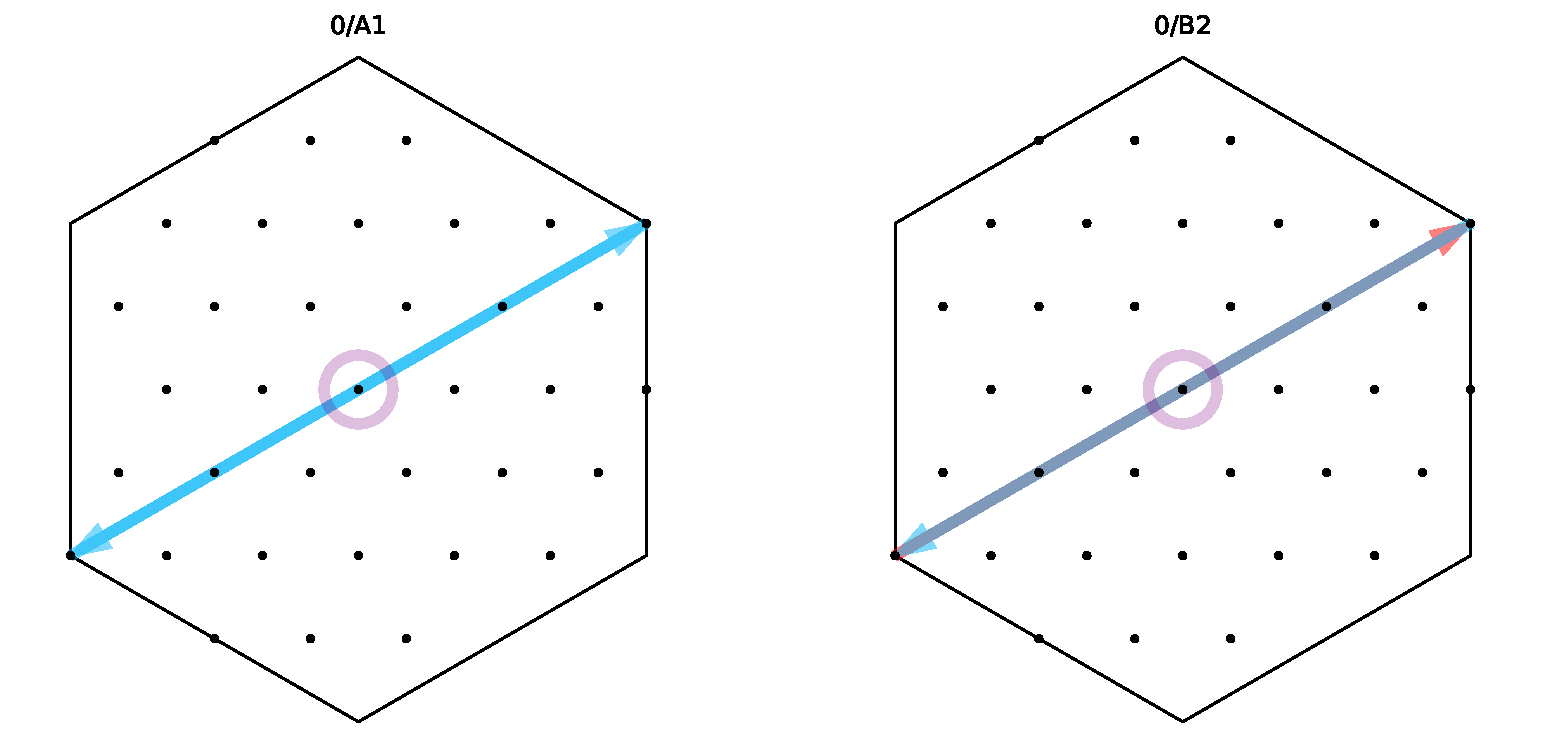
\includegraphics[width=1\linewidth]{BZ_used.pdf}}
  \caption{Momentum shell with two irreducible representations for the available single body momenta. The number on the left side of "/" in the titles indicates the shell, and on the right side is the irreducible representations of the little group. The head of the pink circle shows the total momentum $\Gamma$. Blue/Red arrows point the relative momentum. The color indicates the phase of the operators (red = $\pi$, blue = 0) and the relative thickness indicates the relative weight of that state.}
  \label{fig:used_irrep}
\end{figure}

We will extract the binding energy by independently fitting each correlator. While the data are symmetrical around $\beta/2$, we are allowed to fit a hyperbolic cosine function instead of the exponential function (\cref{eq:fit_exponent}). The method for obtaining the binding energy (\cref{eq:binding_energy}) extracts the energy from one-body correlation function by fitting
\begin{equation}
    f(t) = A\cosh\left(E_0\left(t-\frac{\beta}{2}\right)\right),
    \label{eq:cosh1}
\end{equation}
and then the two-body correlator energy by fitting
\begin{equation}
  f(t) = A\cosh\left(E_0\left(t-\frac{\beta}{2}\right)\right) + C,
    \label{eq:cosh2}
\end{equation}
where $A, E_0, C$ are fit parameters for amplitude, ground energy, and a constant that describes the backward propagating. Note that we are only extracting the ground state energies with these fits. We have tried to add one excited state to the fit, but Python's \textit{curve\_fit} function could not converge at any reasonable maximum step count. Therefore, we should be careful about the range of data points when performing the fits, since we do want to use data only with dominant ground state. We obtain $\Delta E_0$ after subtracting the one-body energies from the two-body.

\begin{figure}[!htbp]
    \begin{subfigure}{.5\textwidth}
      \centering
      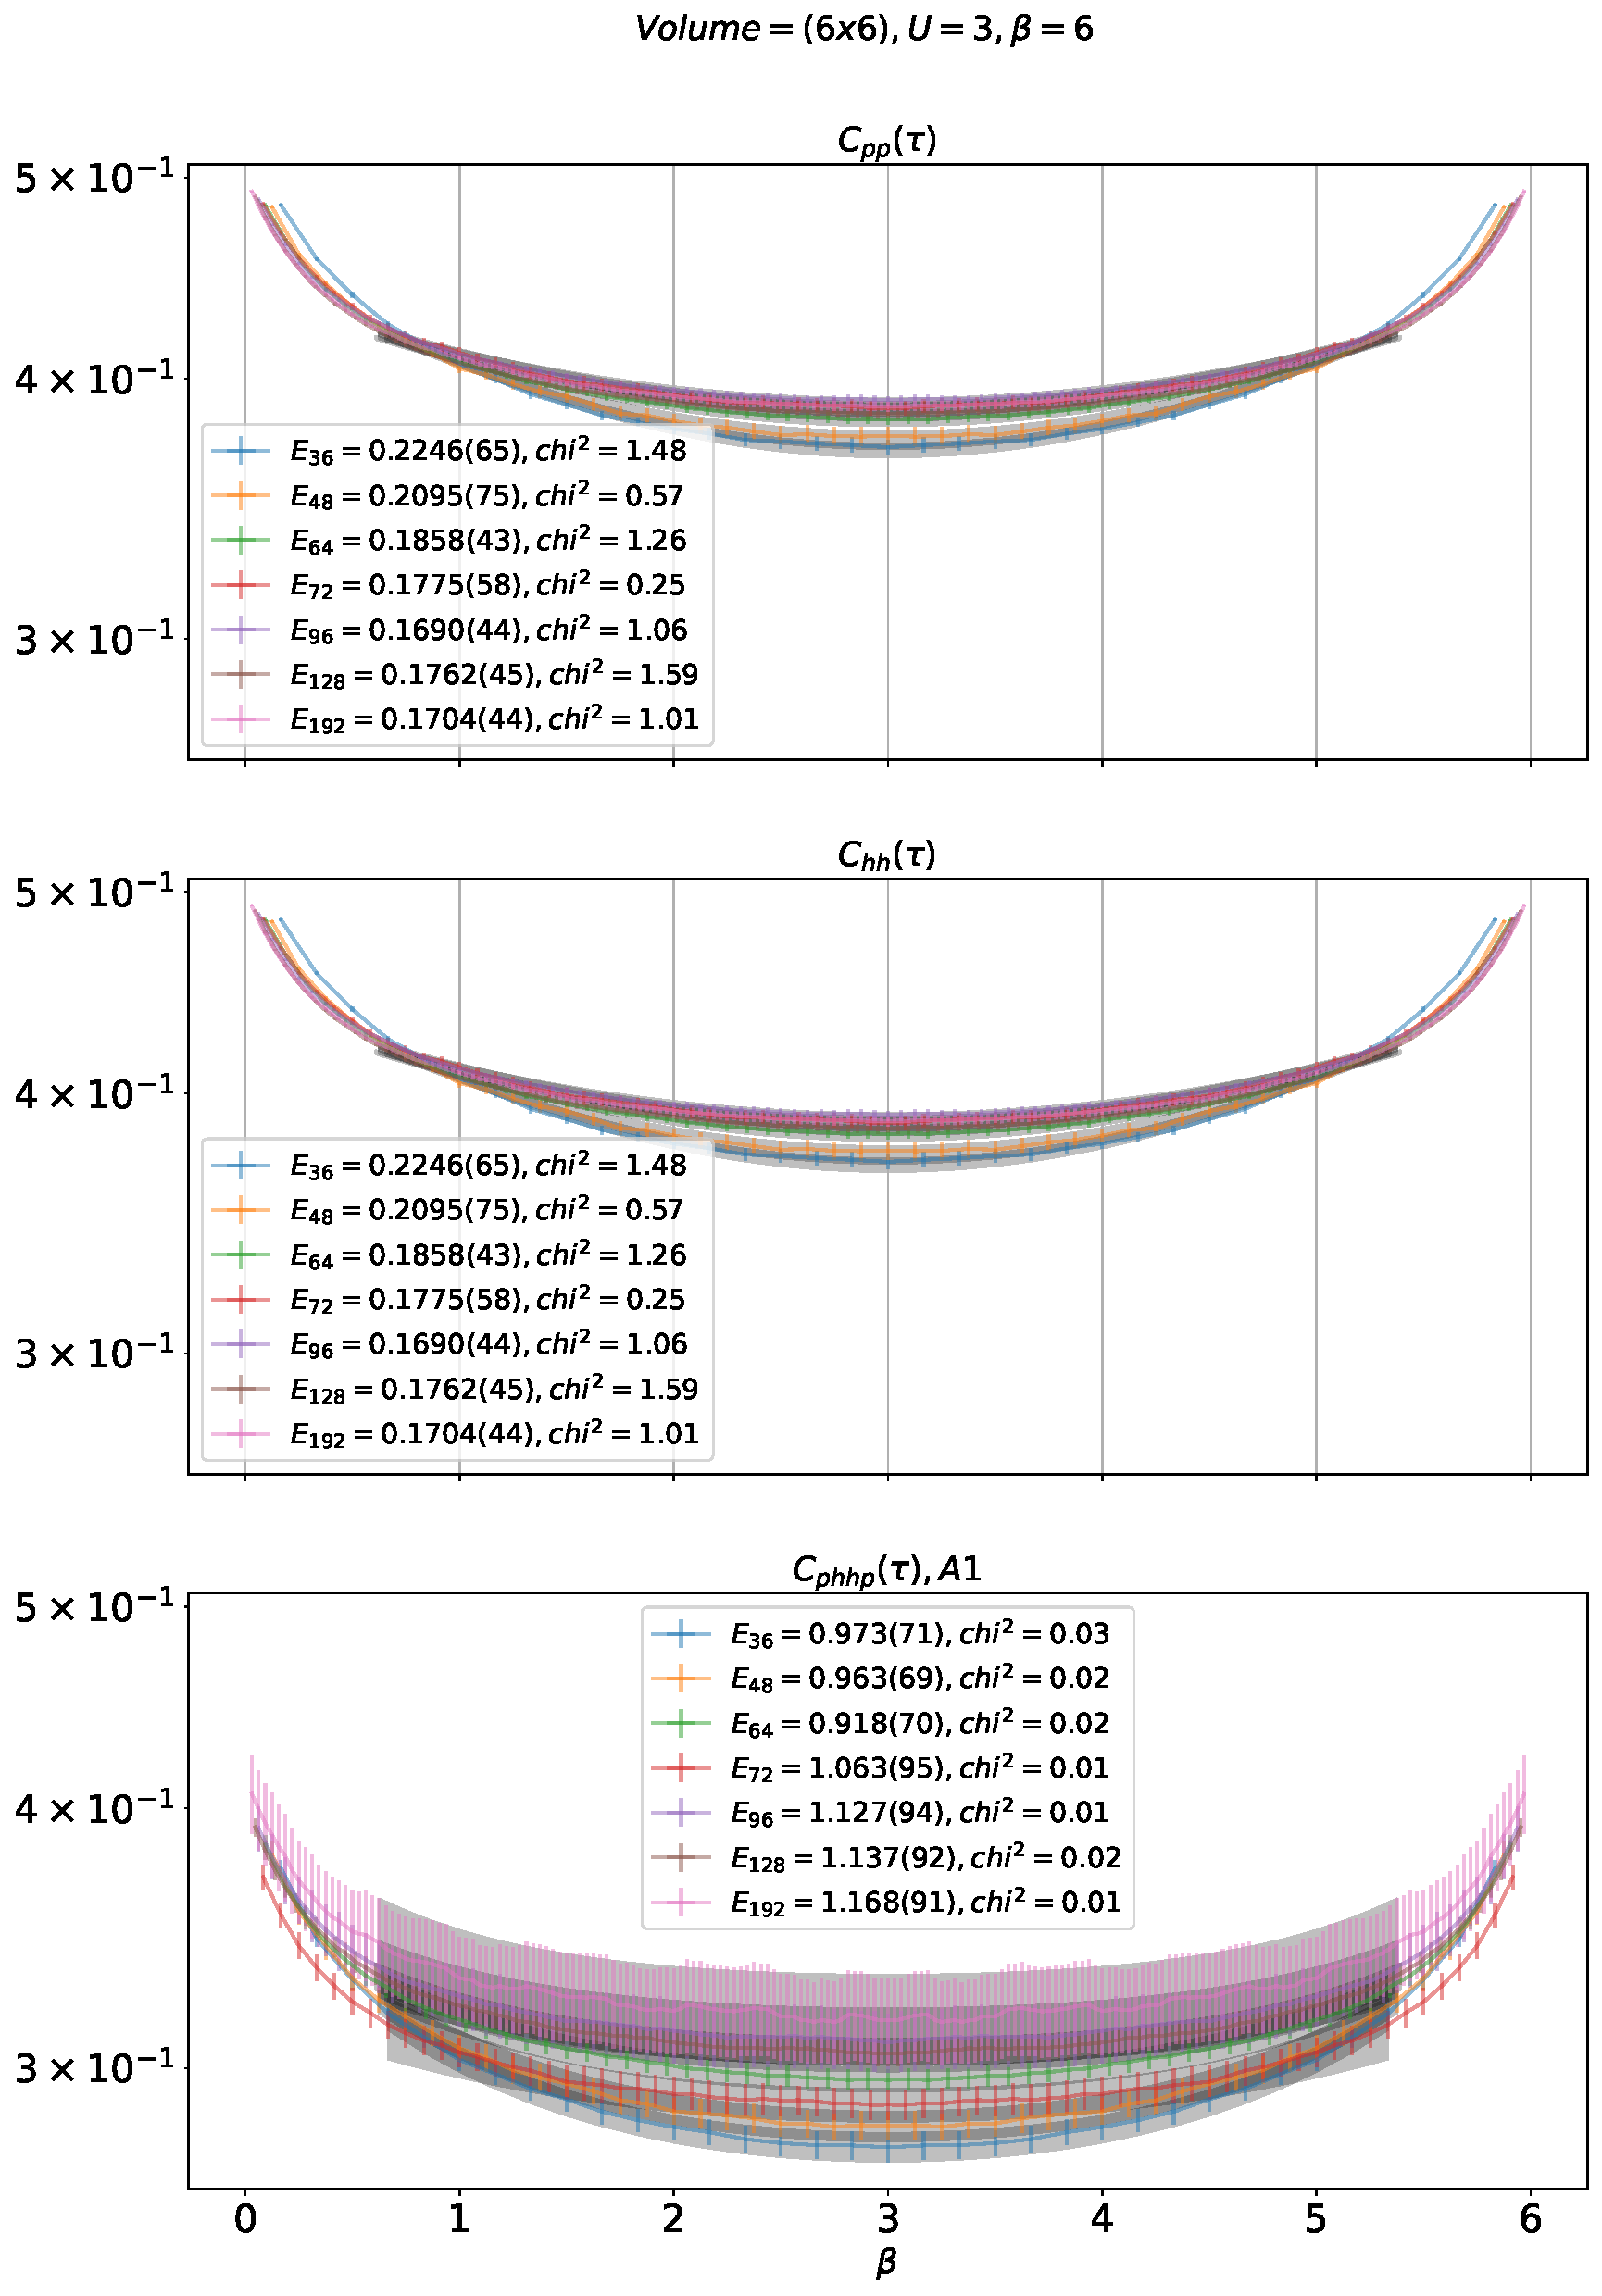
\includegraphics[width=\linewidth]{phhp-0-A1_6x6_U3.0_B6.0.pdf}
    \end{subfigure}%
    \begin{subfigure}{.5\textwidth}
      \centering
      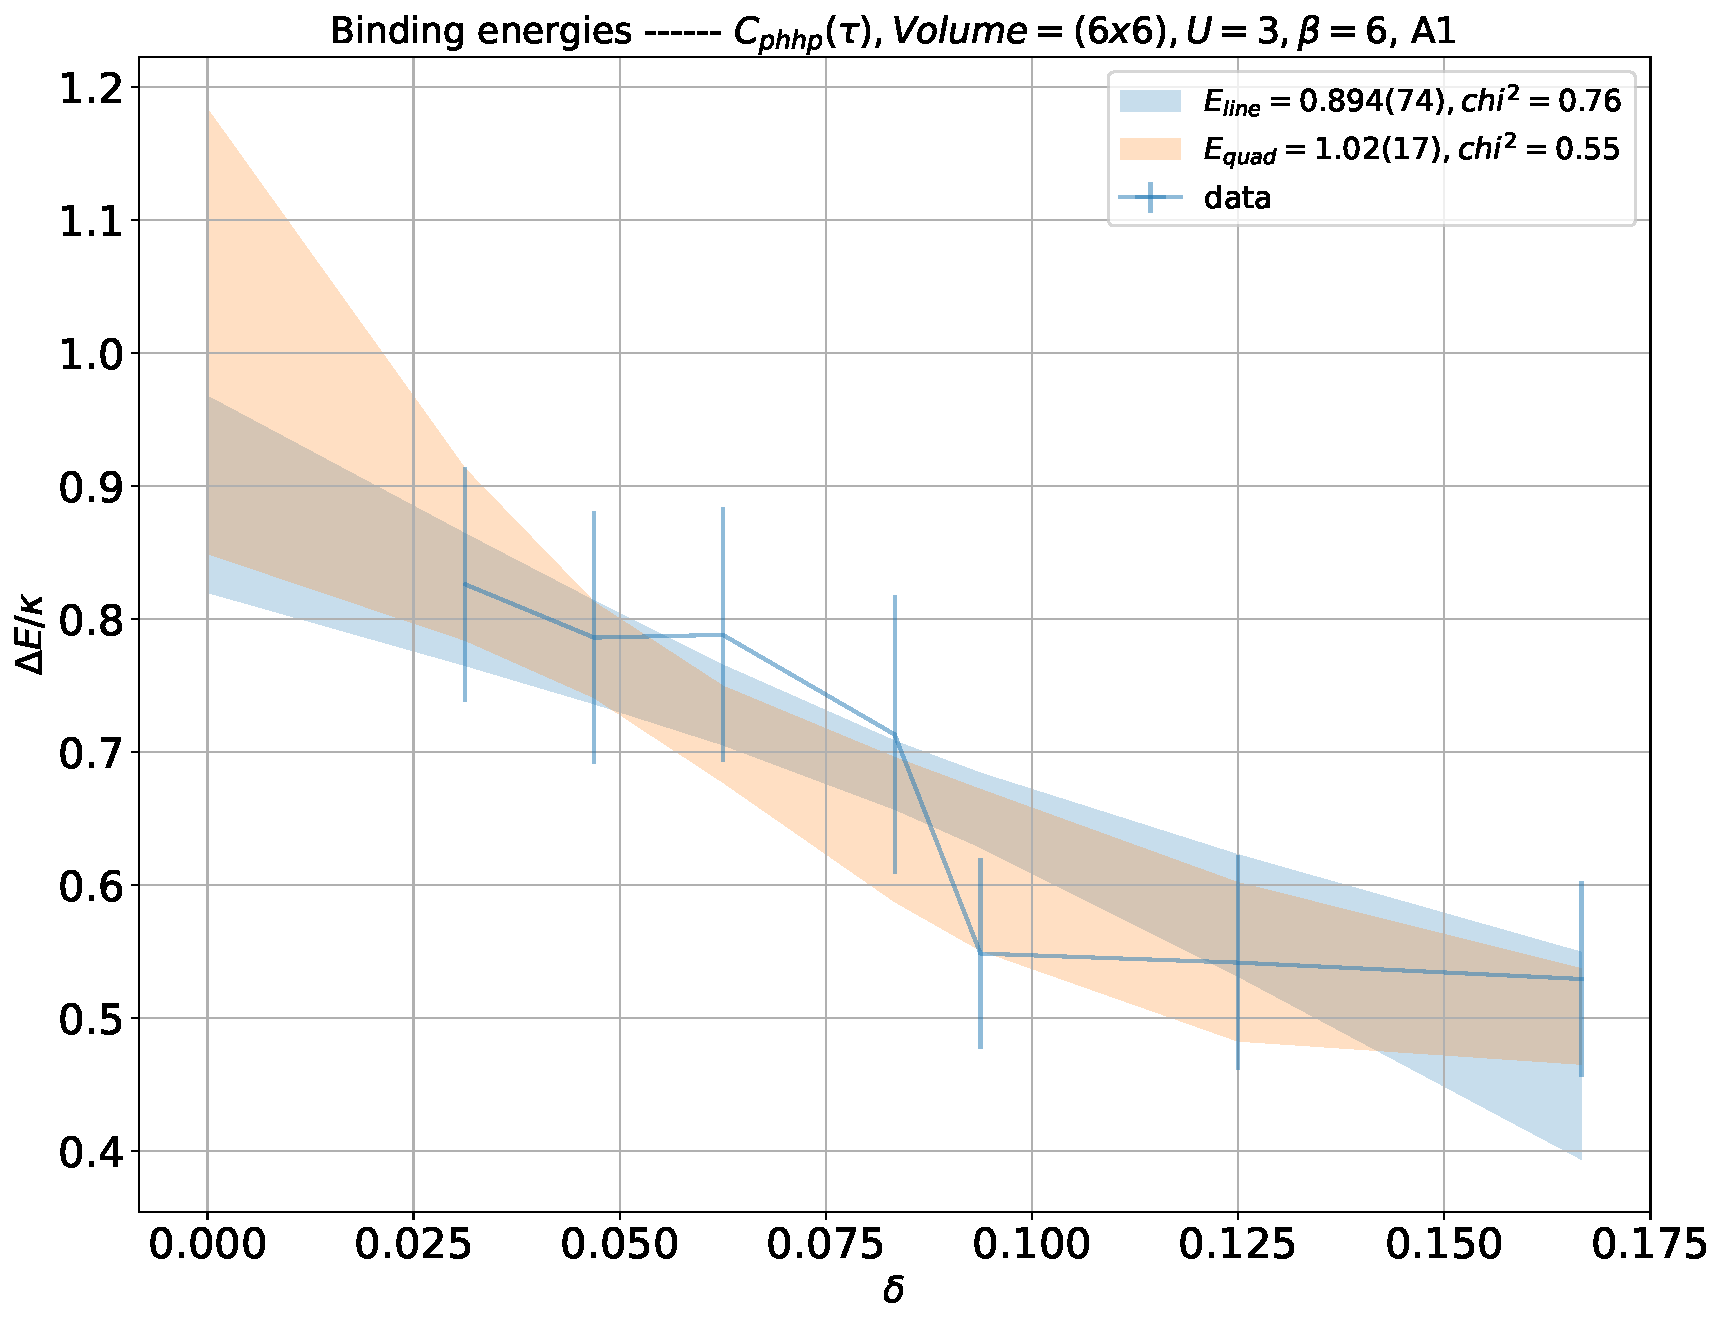
\includegraphics[width=\linewidth]{phhp-0-A1_6x6_U3.0_B6.0_cont.pdf}
    \end{subfigure}
    \caption{An example of how we extract the continuum limit binding energy from the particle-hole correlators. On left we fit one- and two-body correlators for every $N_t$. We fit in $\beta$ range covering the data points with the least excited pollution. This is followed on the right by fitting a linear and a quadratic functions to the $\Delta E_{N_t}$ in order to extrapolate to the continuum limit ($N_t\to\infty$).}
    \label{fig:cont_lim}
\end{figure}

It is shown on \cref{fig:cont_lim}, the fitting of \cref{eq:cosh1} and \cref{eq:cosh2} to one- and two-body correlation functions for all available $N_t$. After which all energies are used to calculate a set of binding energies for each number of time slices $\Delta E_{N_t}$. These energies are then extrapolated to the continuum limit using linear and quadratic functions. This process is repeated for every lattice size, two-body correlation functions, and irreducible representations. All continuum limit extrapolations could be seen in \cref{app:limit}. 

After we have the continuum limit for every lattice size, we can again extrapolate using the same two functions to fit the computed two datasets. The infinite volume results on \cref{fig:u3vol} show that the exciton's binding energy is a positive number for finite temperature and $U=3.0$. Furthermore, the same approximation to the particle-particle correlation functions shows as expected that their binding energy is also positive (\cref{fig:u3vol}). Both irreducible representations have the same behavior. Therefore, we have an evidence to believe that there is not a particle-hole/particle bound state for an infinite volume at finite temperature and $U=3.0$.
\begin{figure}[!htbp]
  \begin{subfigure}{.5\textwidth}
    \centering
    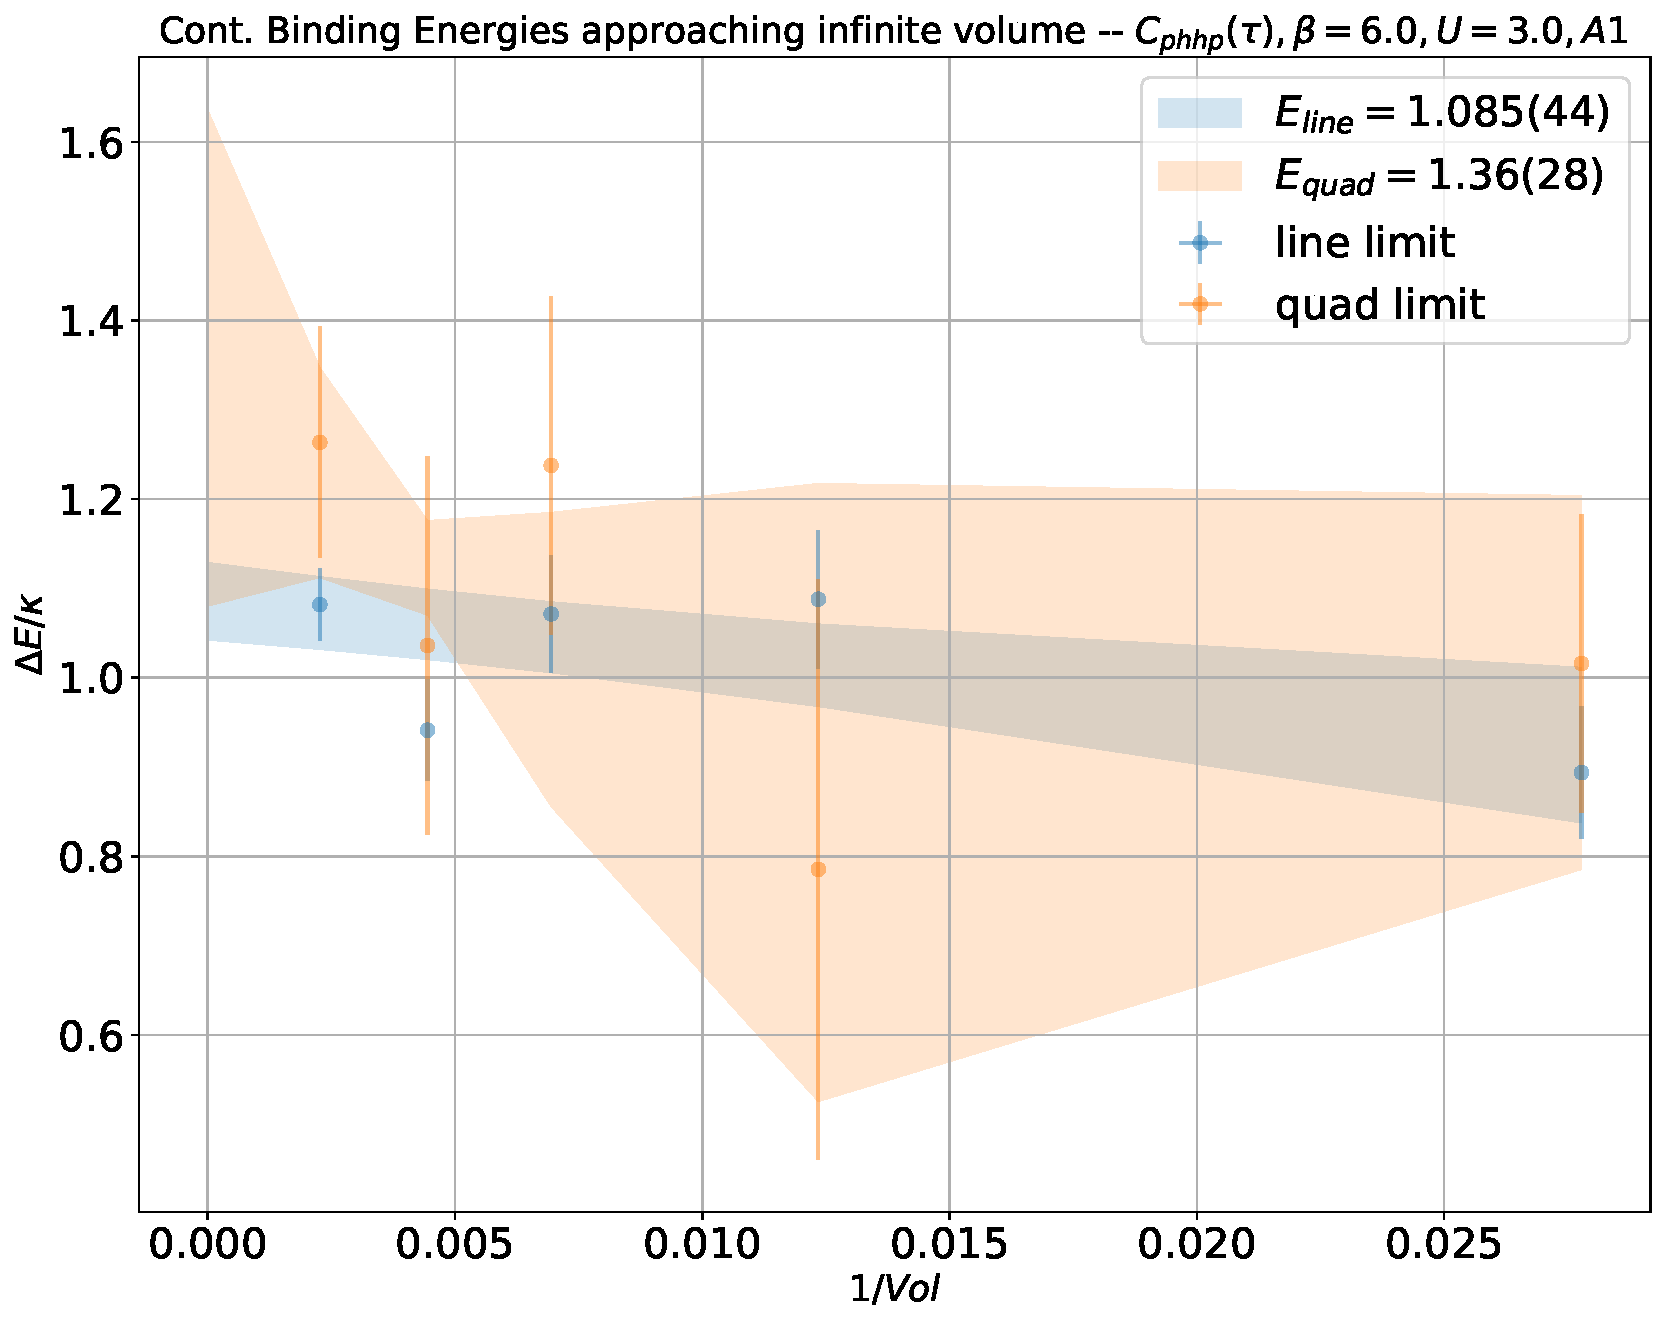
\includegraphics[width=\linewidth]{phhp-0-A1_21x21_U3_B6_vol.pdf}
  \end{subfigure}%
  \begin{subfigure}{.5\textwidth}
    \centering
    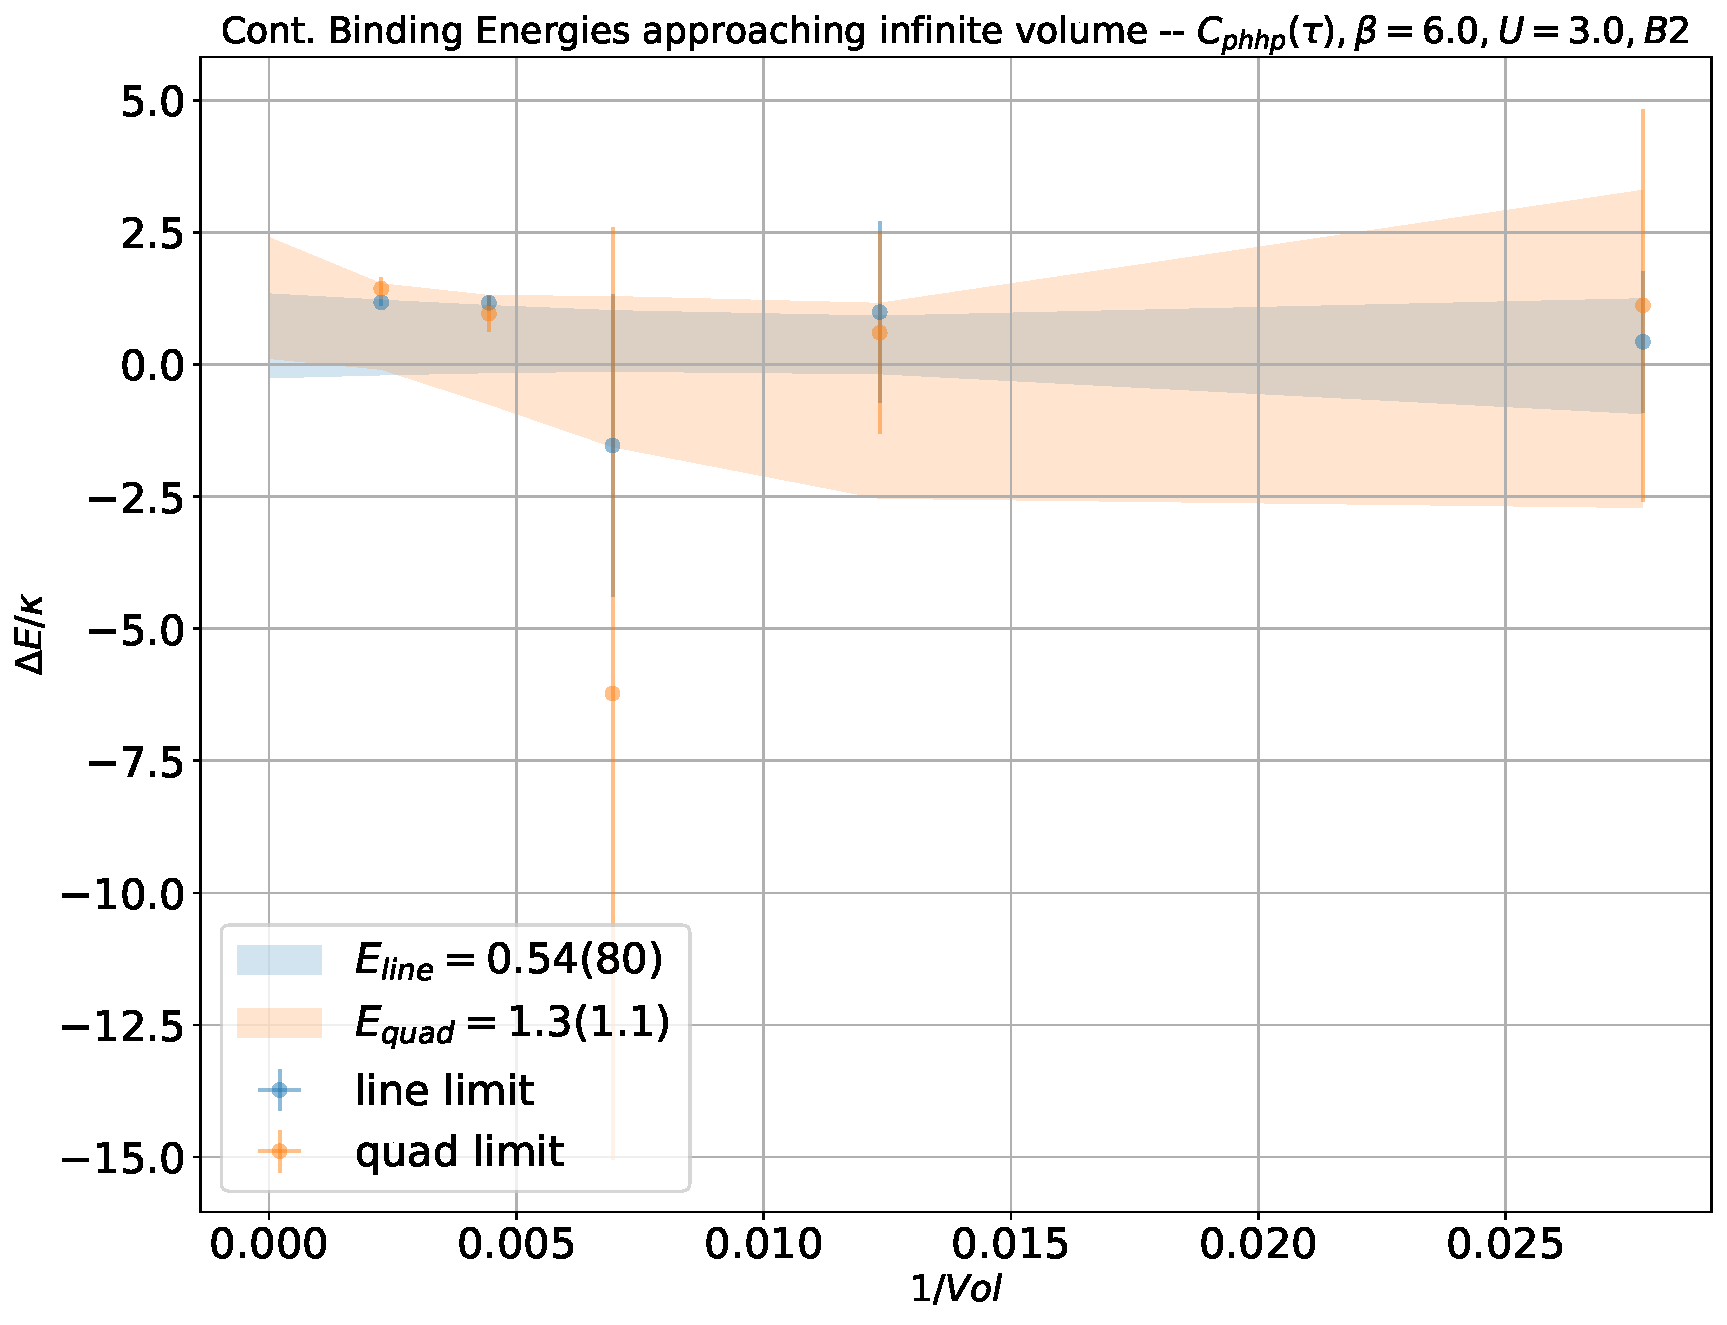
\includegraphics[width=\linewidth]{phhp-0-B2_21x21_U3_B6_vol.pdf}
  \end{subfigure}
  \begin{subfigure}{.5\textwidth}
      \centering
      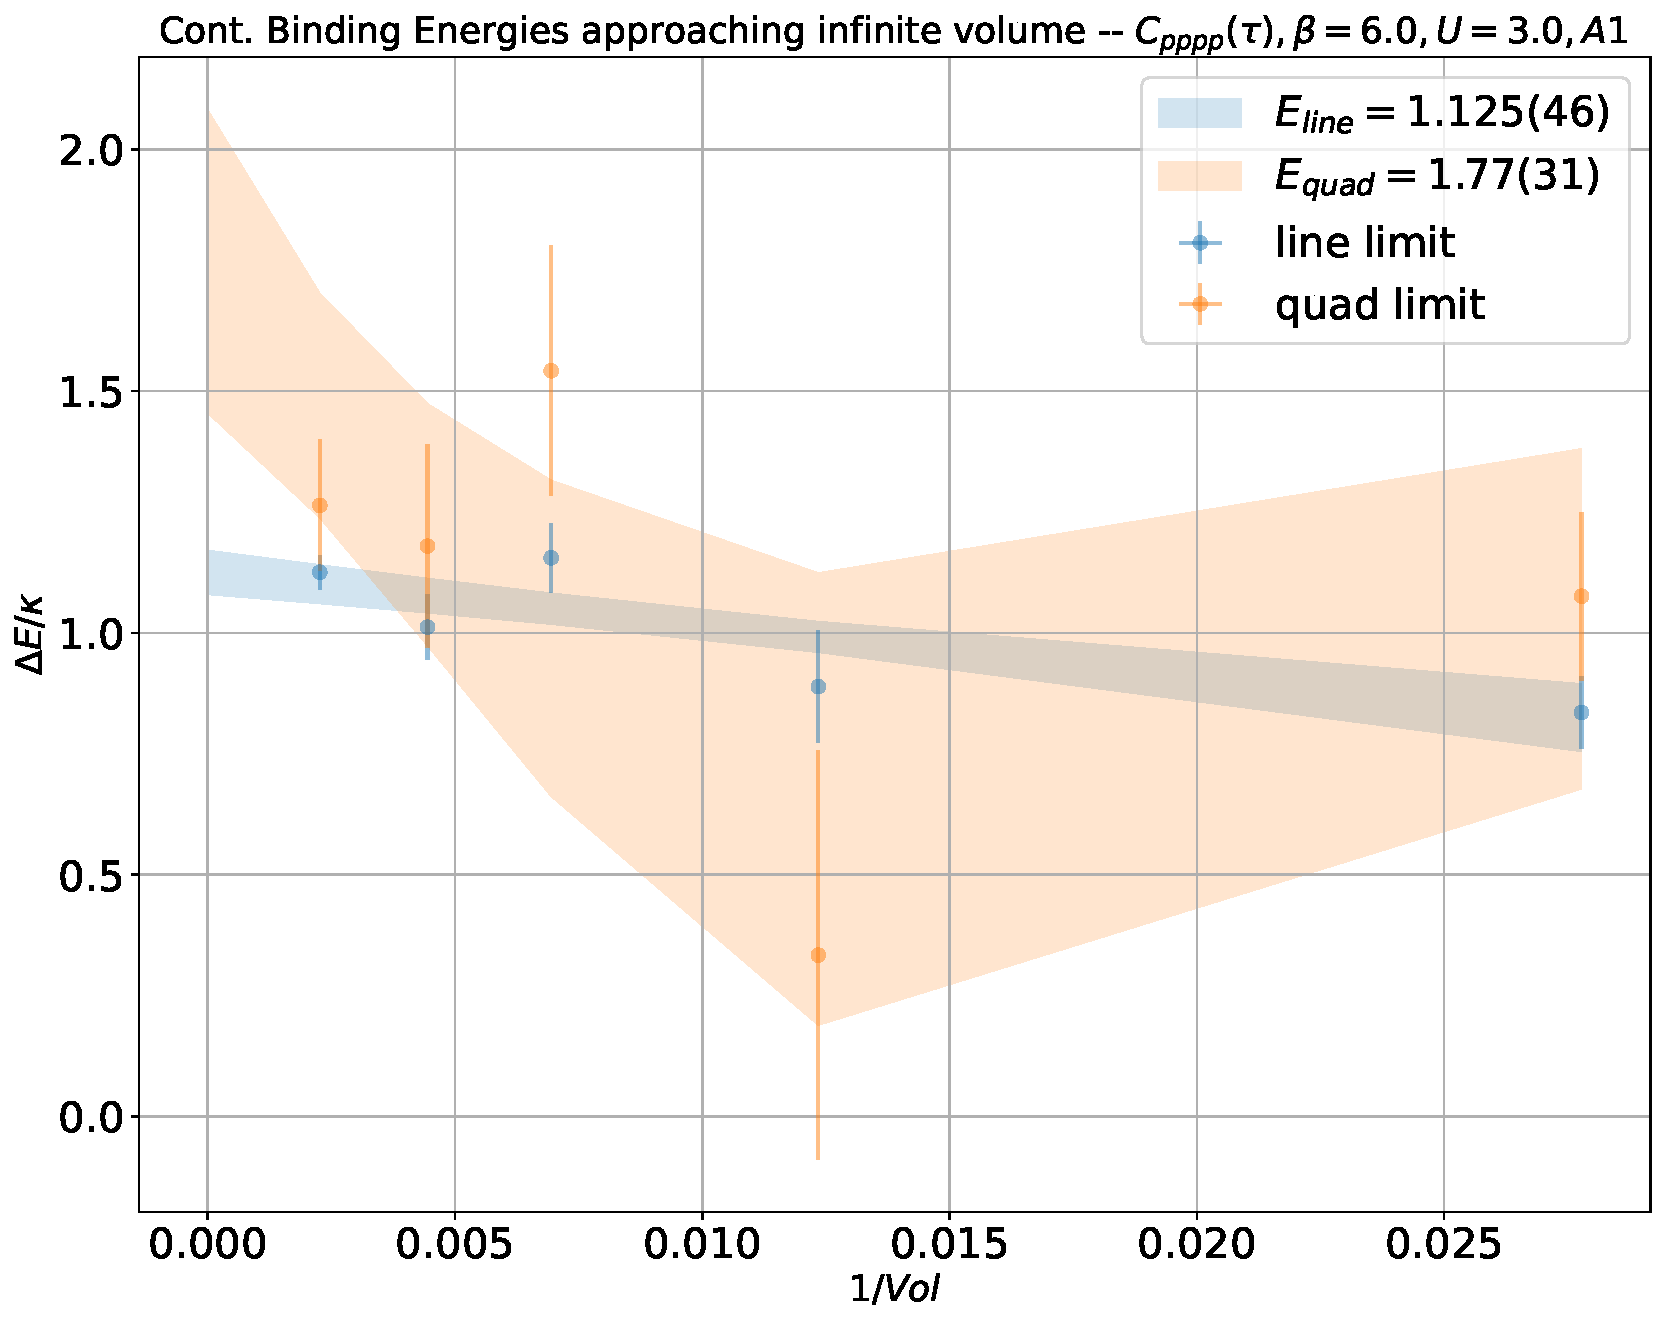
\includegraphics[width=\linewidth]{pppp-0-A1_21x21_U3_B6_vol.pdf}
  \end{subfigure}
  \begin{subfigure}{.5\textwidth}
      \centering
      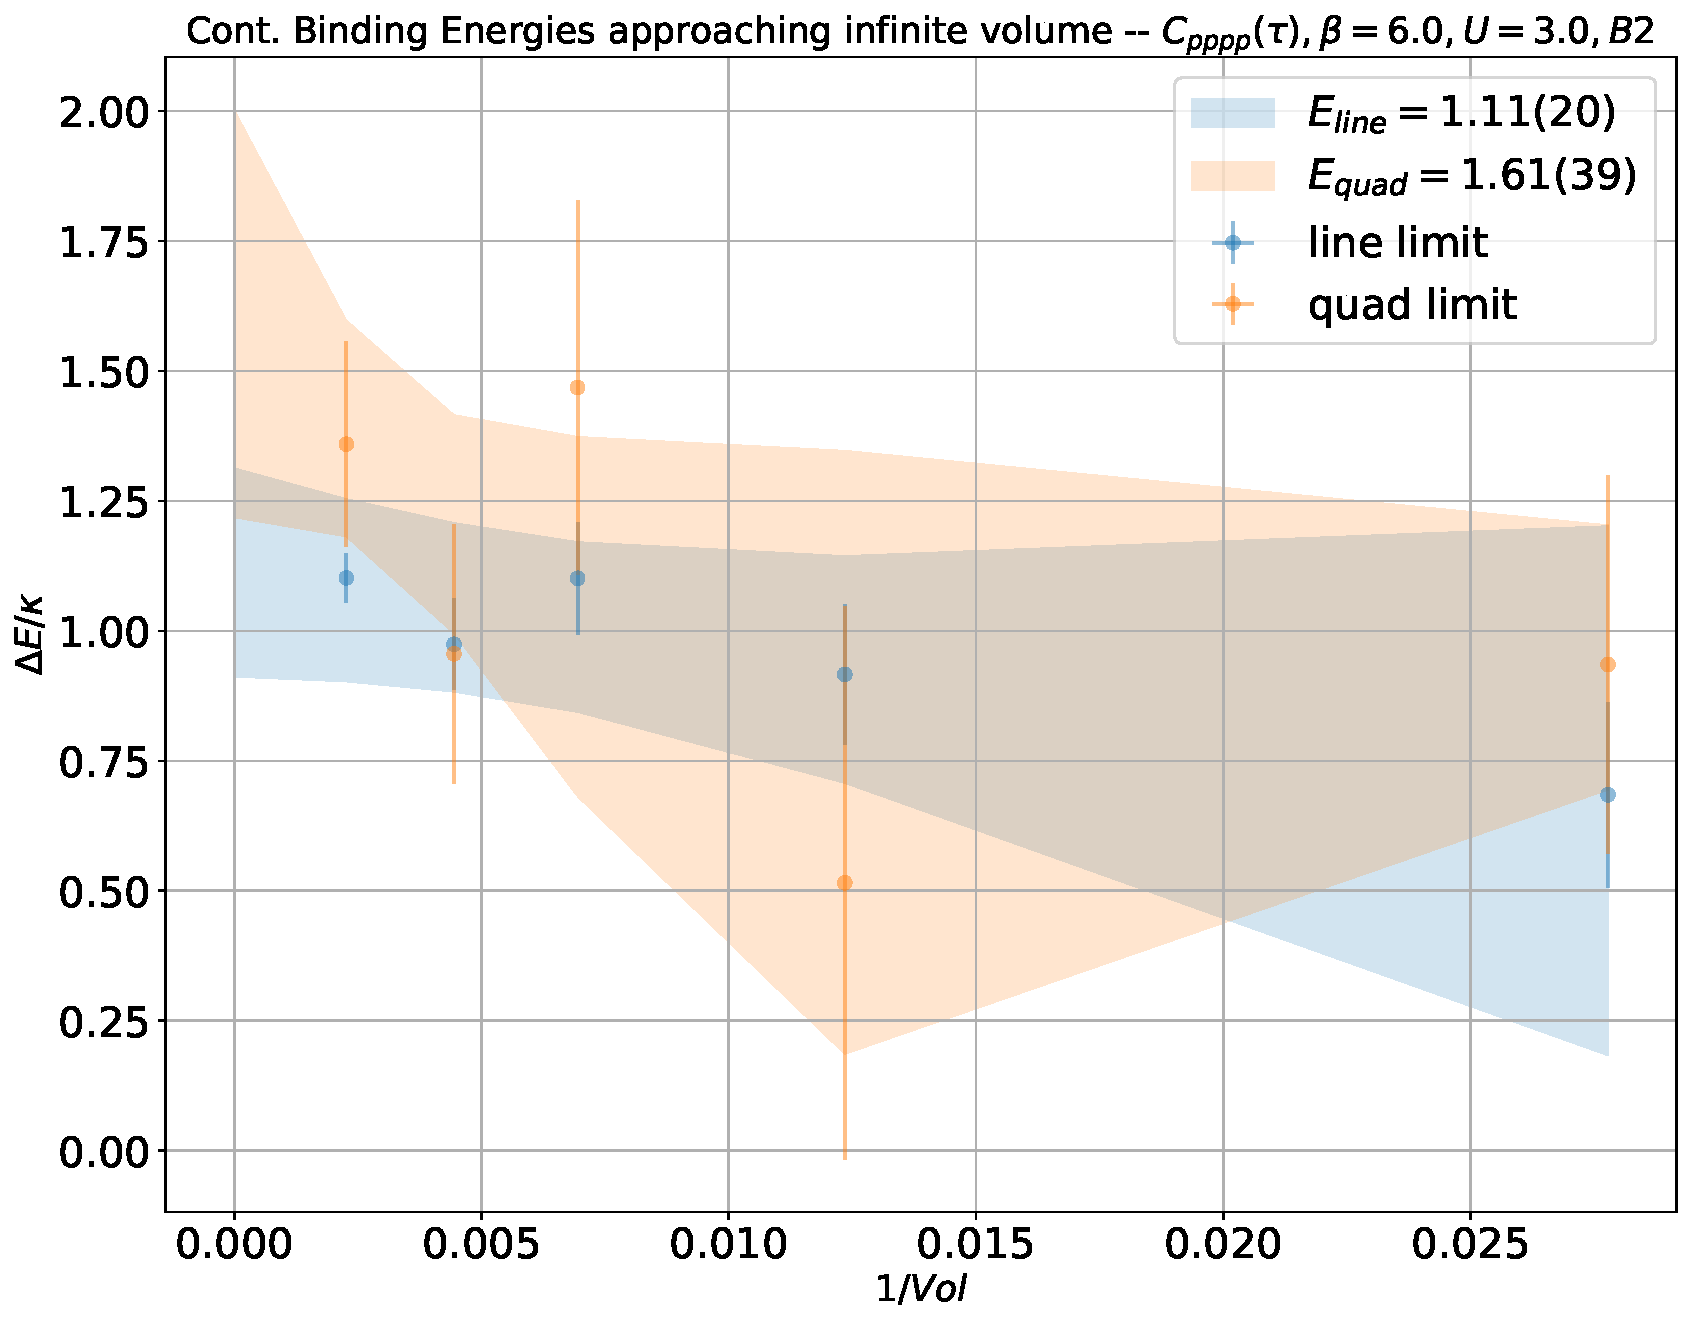
\includegraphics[width=\linewidth]{pppp-0-B2_21x21_U3_B6_vol.pdf}
  \end{subfigure}
  \caption{Infinite volume extrapolation of continuum limit binding energies for $C_{phhp}$ and $C_{pppp}$. This is done at $\beta=6.0$ and both irreducible representations. We plot it as a function of $1/Vol$ because it is simpler to show where the limit lies.}
  \label{fig:u3vol}
\end{figure}

The results for $\Delta E_{phhp}$ and $\Delta E_{pppp}$ at $V\to\infty$ show a small scaling when extrapolating of the infinite volume. This means that we can fit and extrapolate our data to the continuum limit followed by the zero temperature limit at finite volume. We can assume that the result we get, is in the vicinity of the true value, but with an extra added systematic error. From the available ensembles (\cref{tab:work_ensembles}), we could not only get results for $U=3.0$ but also for $U=4.0$, which is on the other side of the critical coupling $U_{crit}\approx 3.85$. Correlation functions for $\beta = 3.0$ are omitted when performing the zero-temperature approximation because they have proved too noisy and the extracted energy is unreliable. All plots reaching the continuum limit are shown in \cref{app:limit} (\crefrange{fig:fig11}{fig:fig20}). Here, we will show only the final extrapolations for both correlation functions at both couplings and irreducible representations.  
\begin{figure}[!htbp]
    \begin{subfigure}{.5\textwidth}
      \centering
      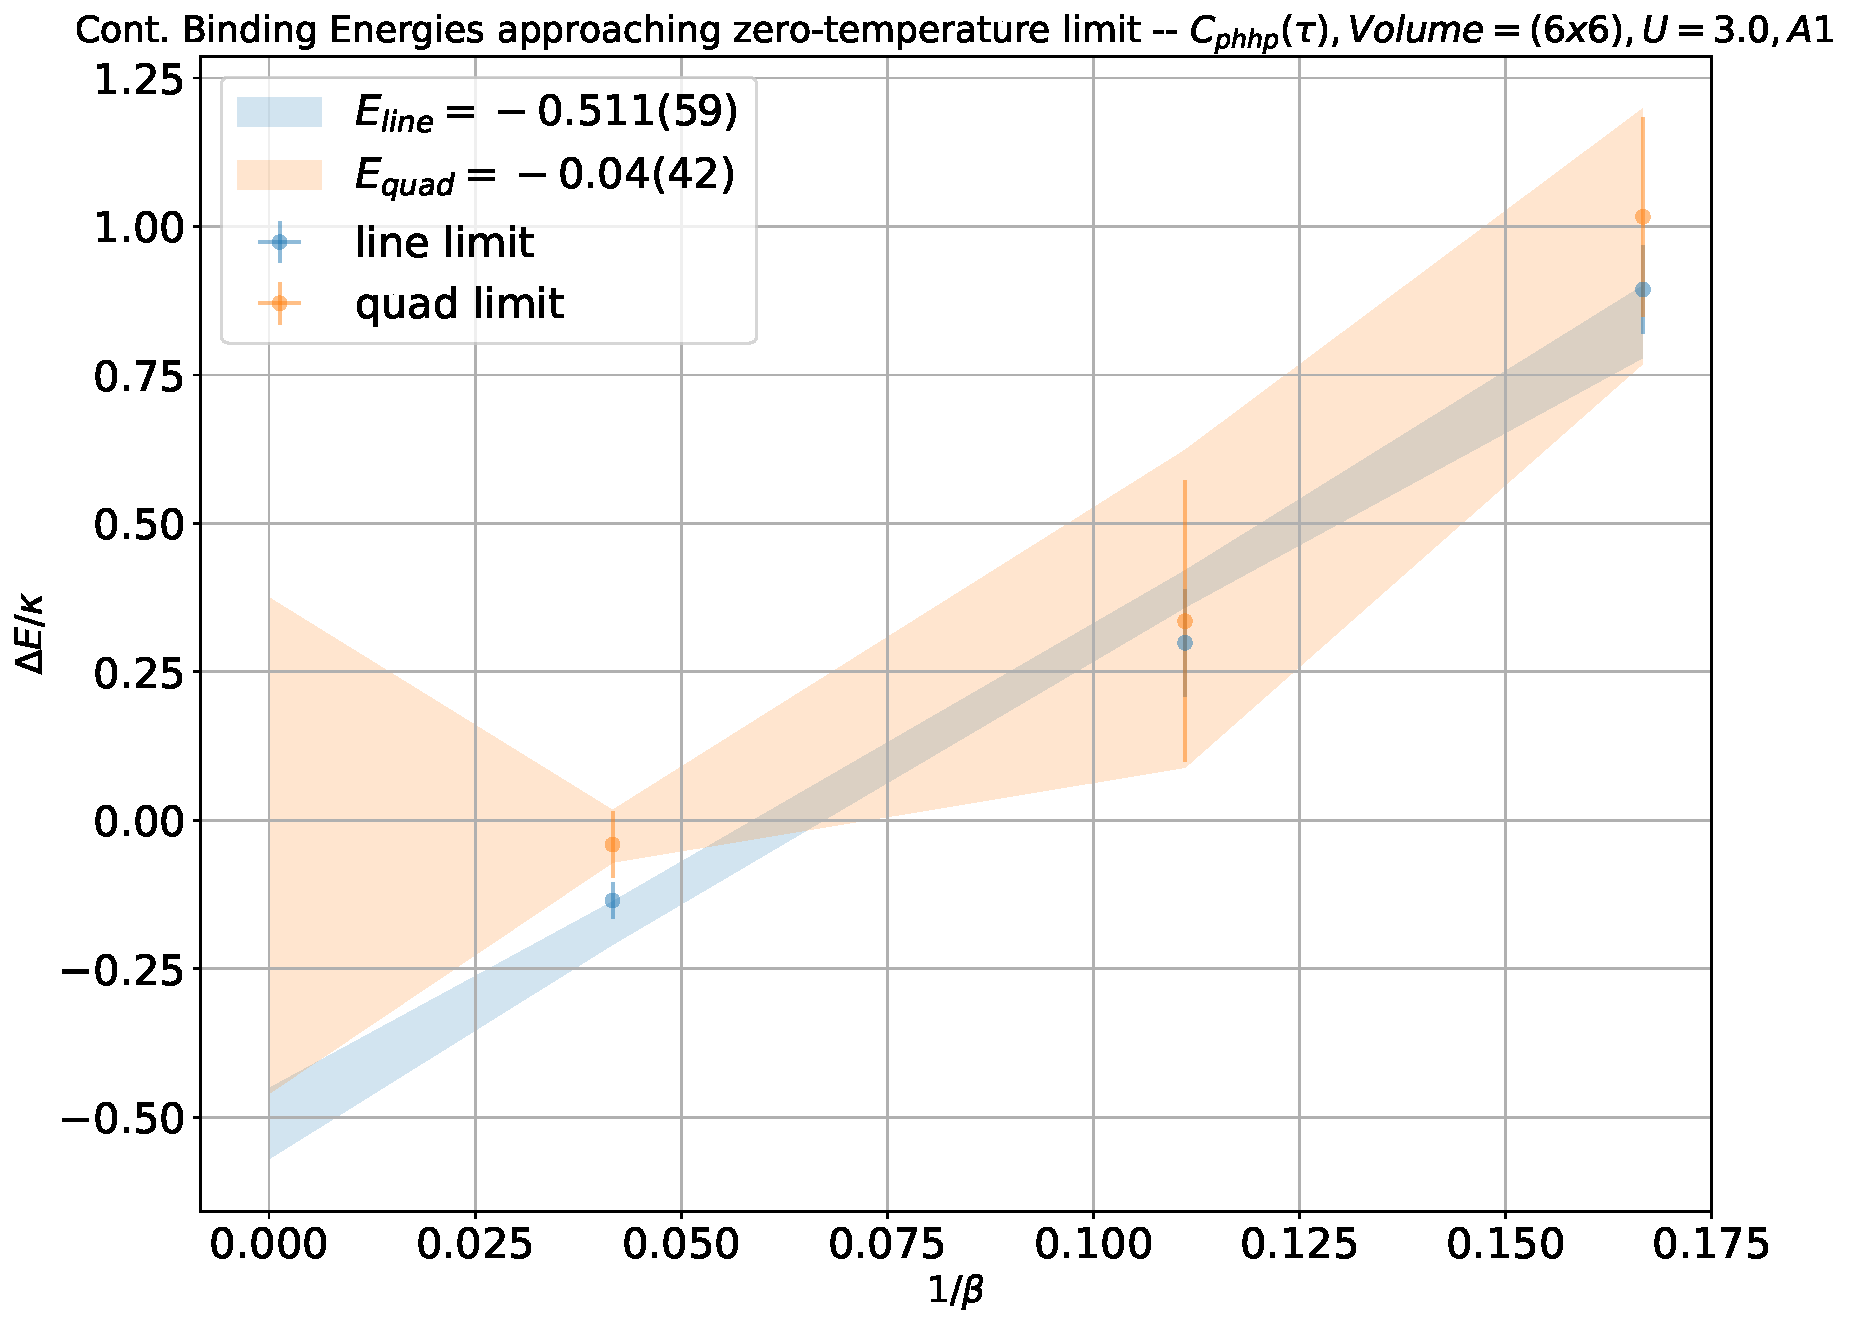
\includegraphics[width=\linewidth]{phhp-0-A1_6x6_U3.0_B24.0_temp.pdf}
    \end{subfigure}%
    \begin{subfigure}{.5\textwidth}
      \centering
      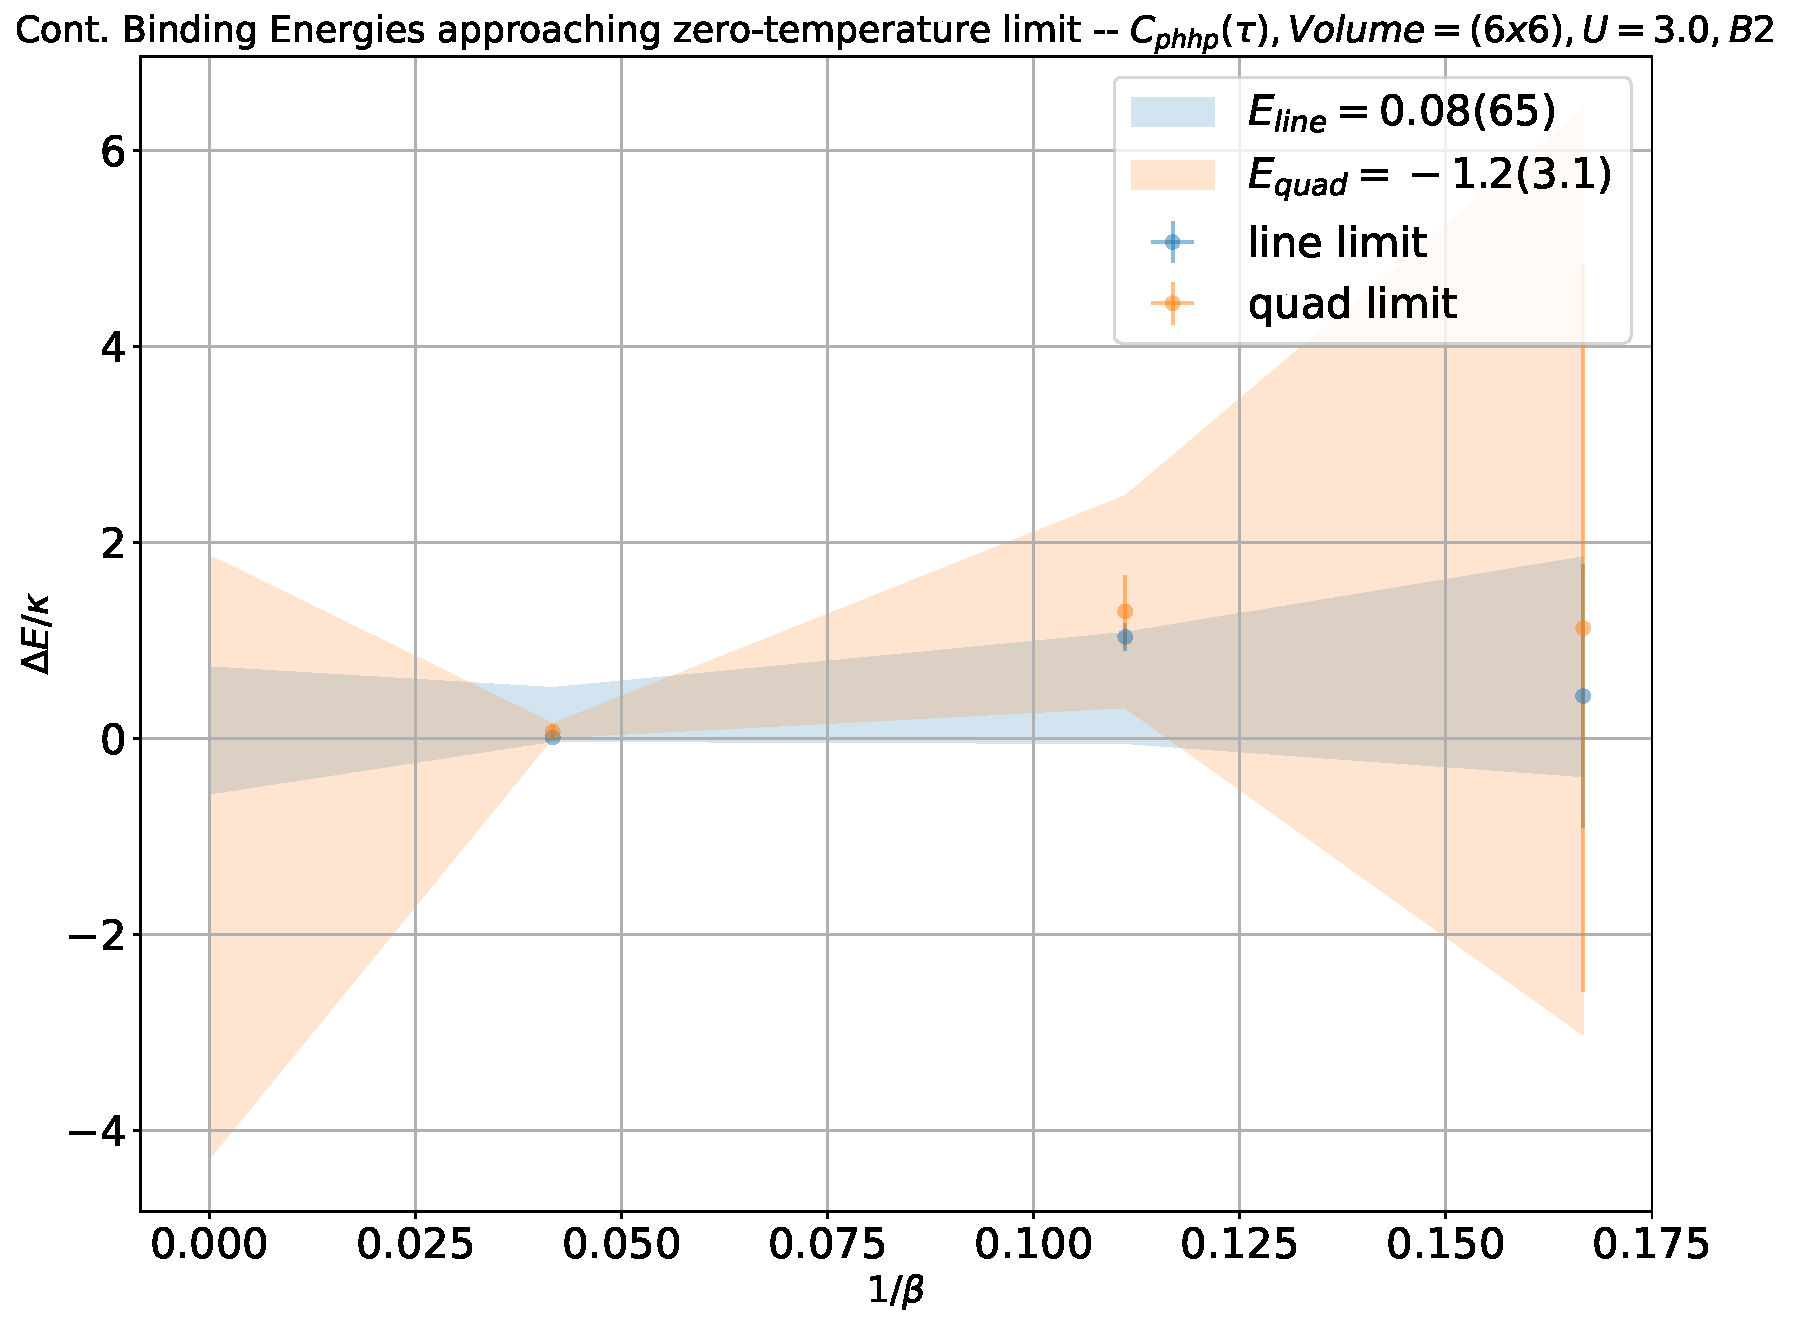
\includegraphics[width=\linewidth]{phhp-0-B2_6x6_U3.0_B24.0_temp.pdf}
    \end{subfigure}
    \begin{subfigure}{.5\textwidth}
        \centering
        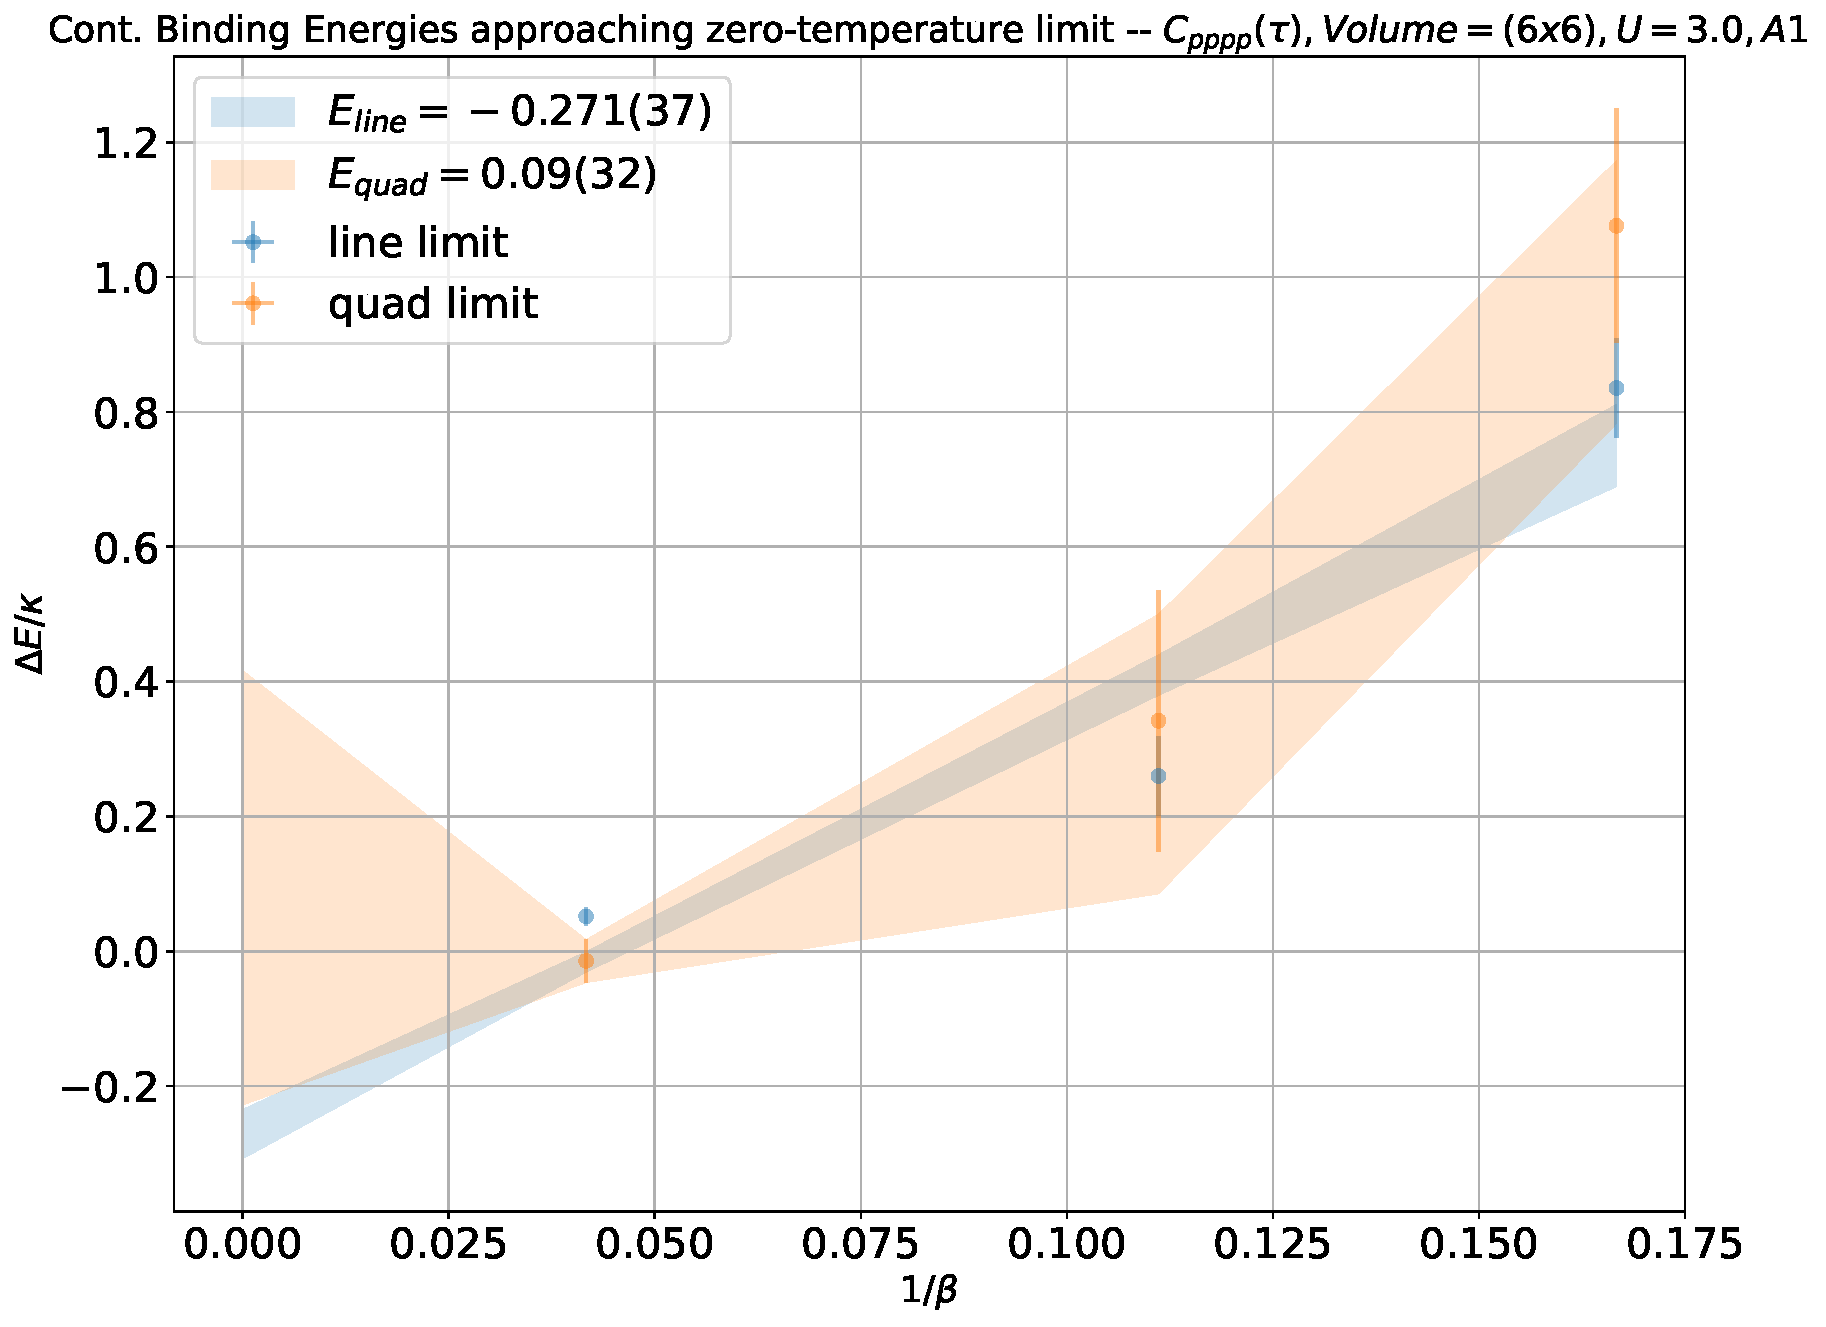
\includegraphics[width=\linewidth]{pppp-0-A1_6x6_U3.0_B24.0_temp.pdf}
    \end{subfigure}
    \begin{subfigure}{.5\textwidth}
        \centering
        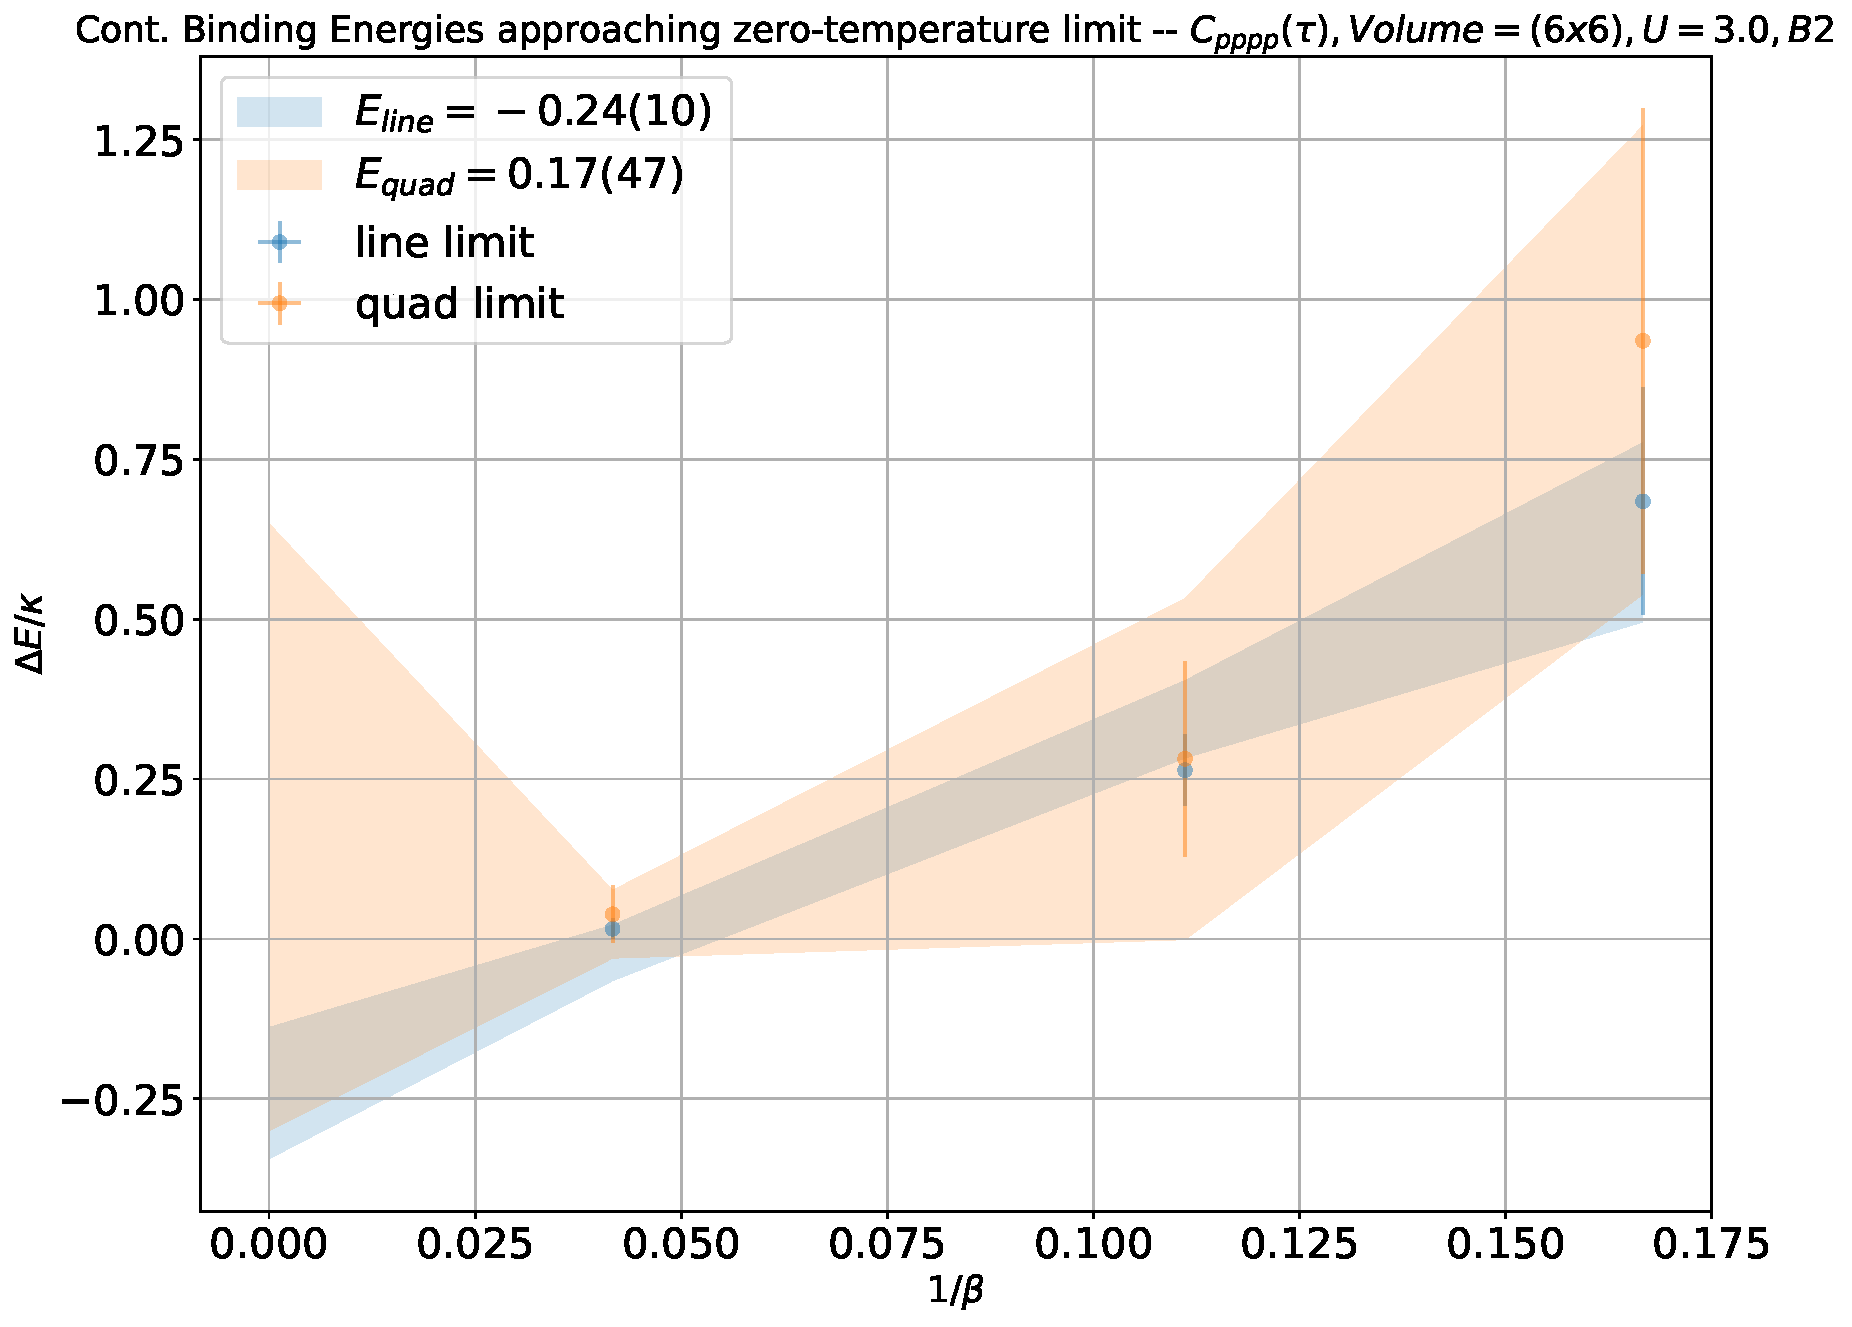
\includegraphics[width=\linewidth]{pppp-0-B2_6x6_U3.0_B24.0_temp.pdf}
    \end{subfigure}
    \caption{Zero-temperature extrapolation of continuum limit binding energies for $C_{phhp}$ and $C_{pppp}$ and both irreducible representations. This is done at lattice size $(6\times 6)$ and $U=3.0$. We plot it as a function of $1/\beta$ because it is simpler to show where the limit lies.}
    \label{fig:u3temp}
  \end{figure}
The results for $U=3.0$ (\cref{fig:u3temp}) show that the zero-temperature binding energy of the exciton as well as the particle pair is close to zero or negative for both irreducible representations, depending on which extrapolation function is better approximating the limit. Thus, an investigation with more $\beta$ data points must be performed.
\begin{figure}[!htbp]
    \begin{subfigure}{.5\textwidth}
      \centering
      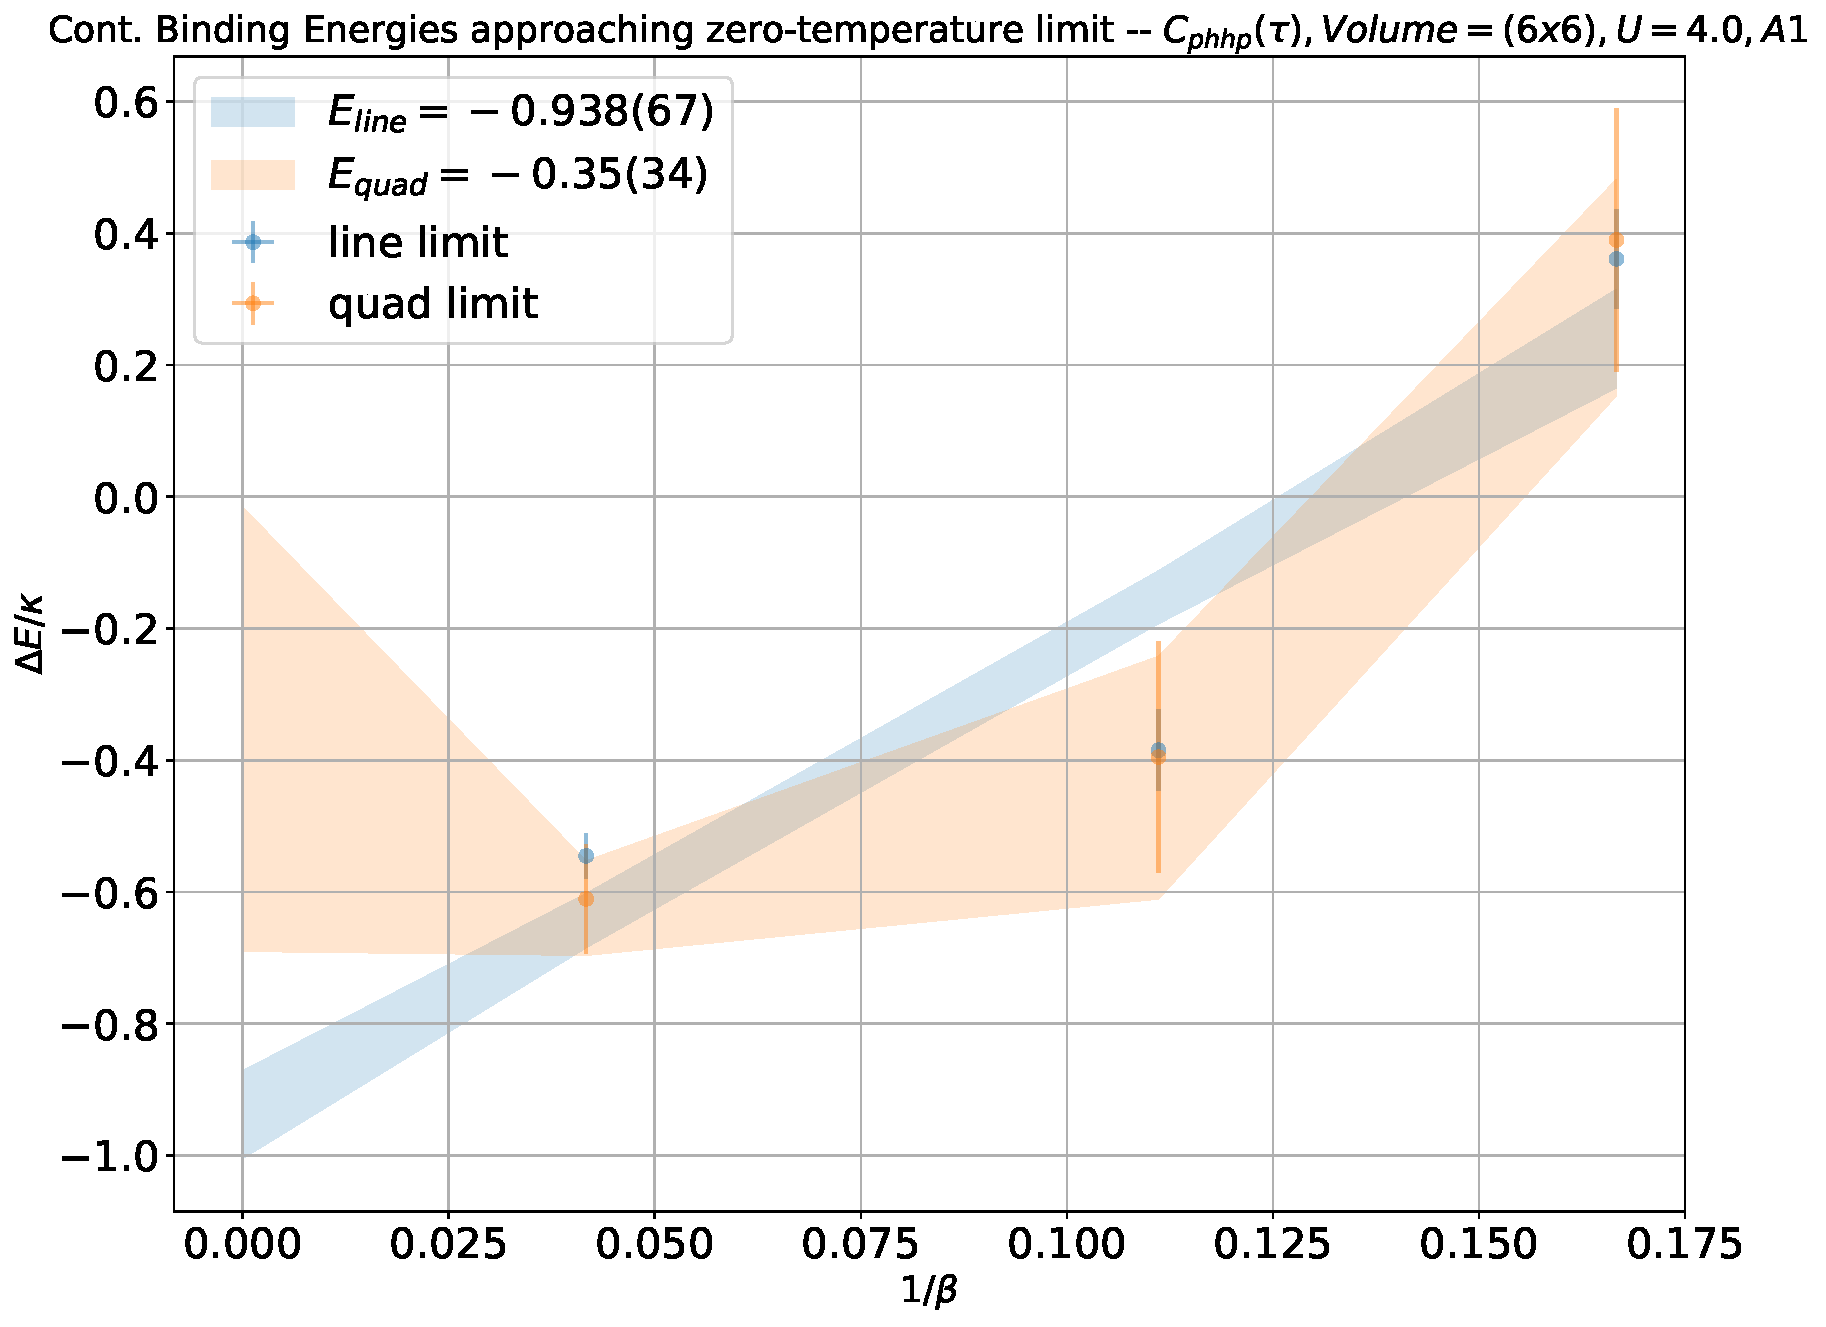
\includegraphics[width=\linewidth]{phhp-0-A1_6x6_U4.0_B24.0_temp.pdf}
    \end{subfigure}%
    \begin{subfigure}{.5\textwidth}
      \centering
      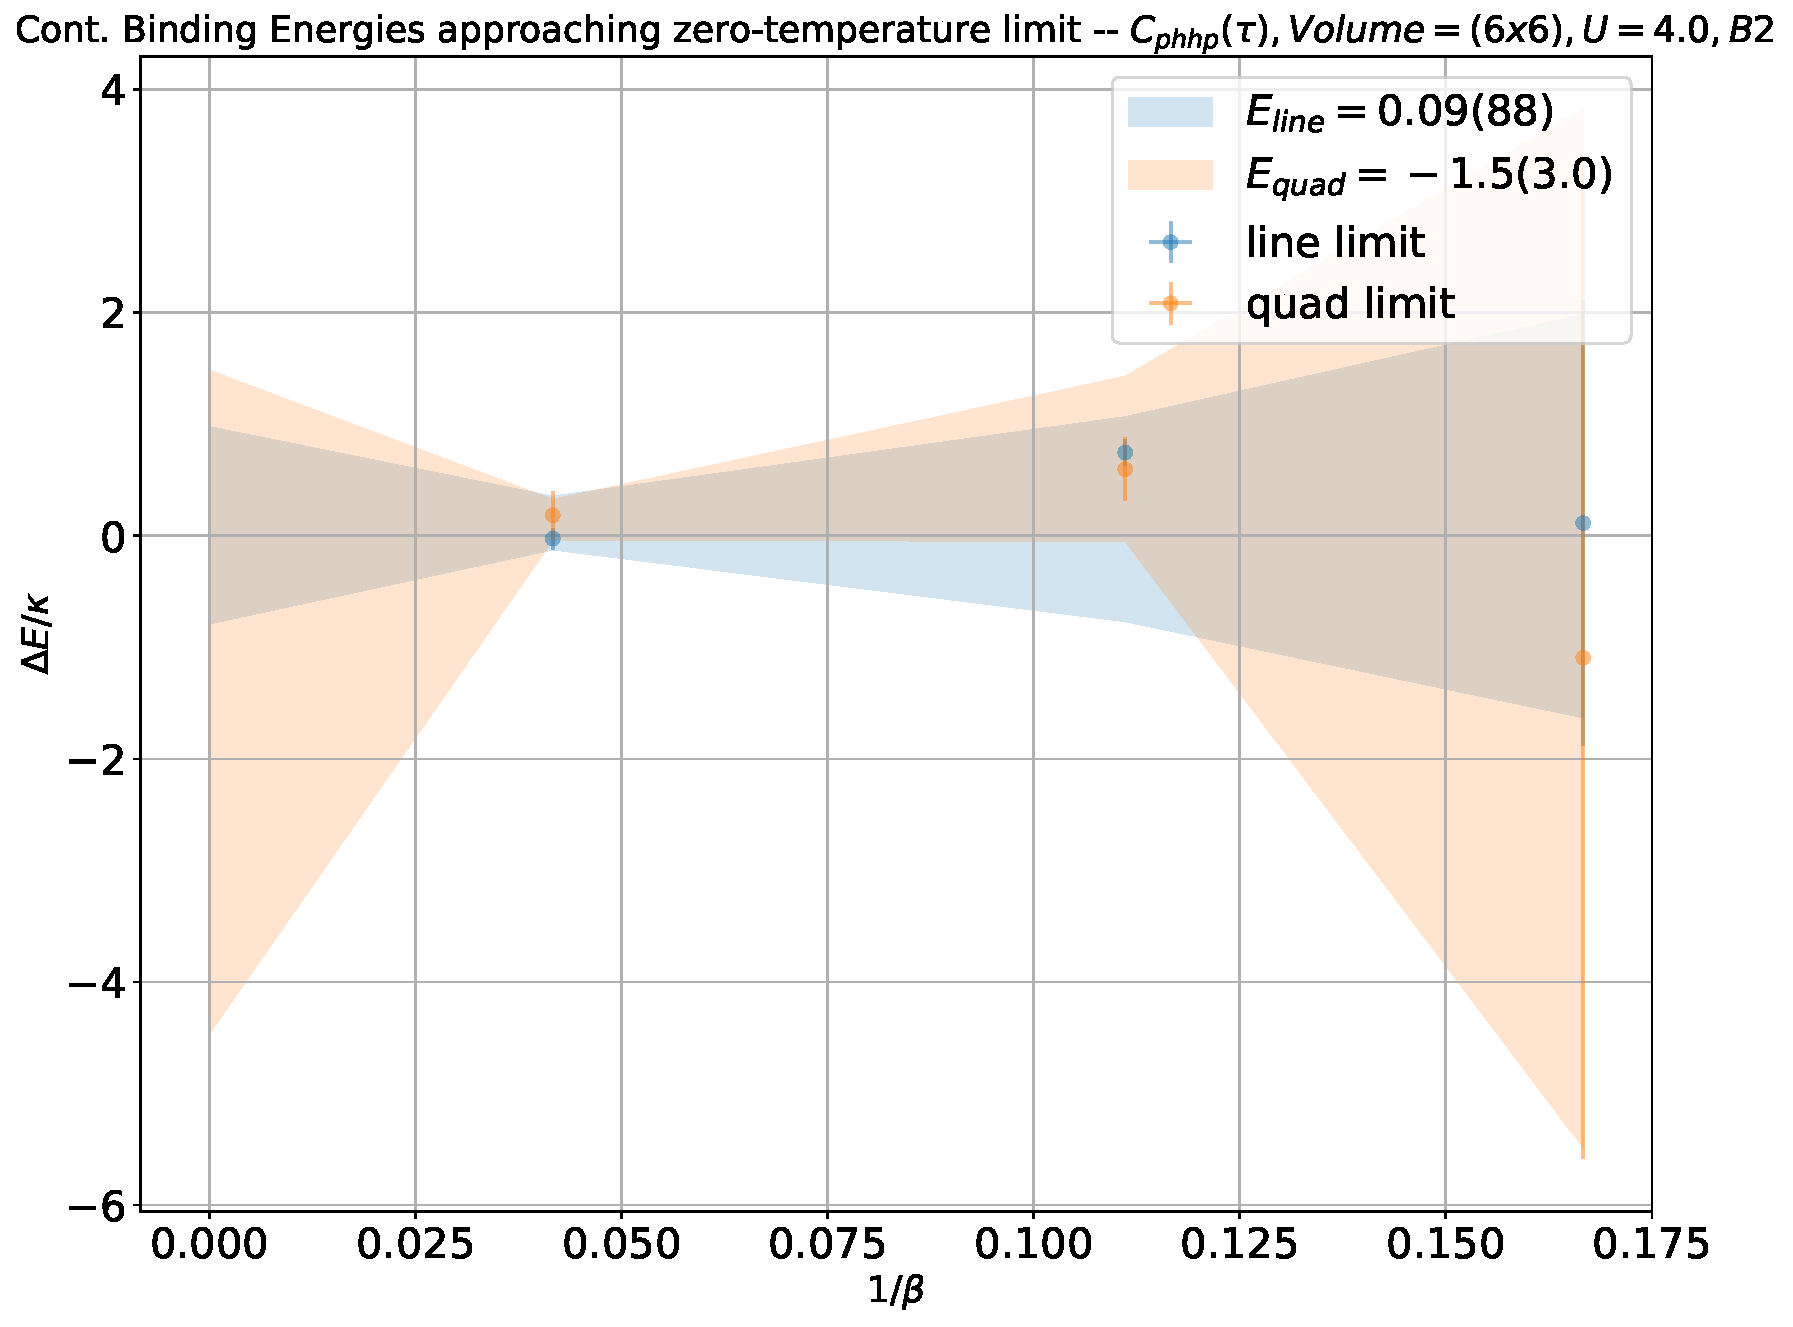
\includegraphics[width=\linewidth]{phhp-0-B2_6x6_U4.0_B24.0_temp.pdf}
    \end{subfigure}
    \begin{subfigure}{.5\textwidth}
        \centering
        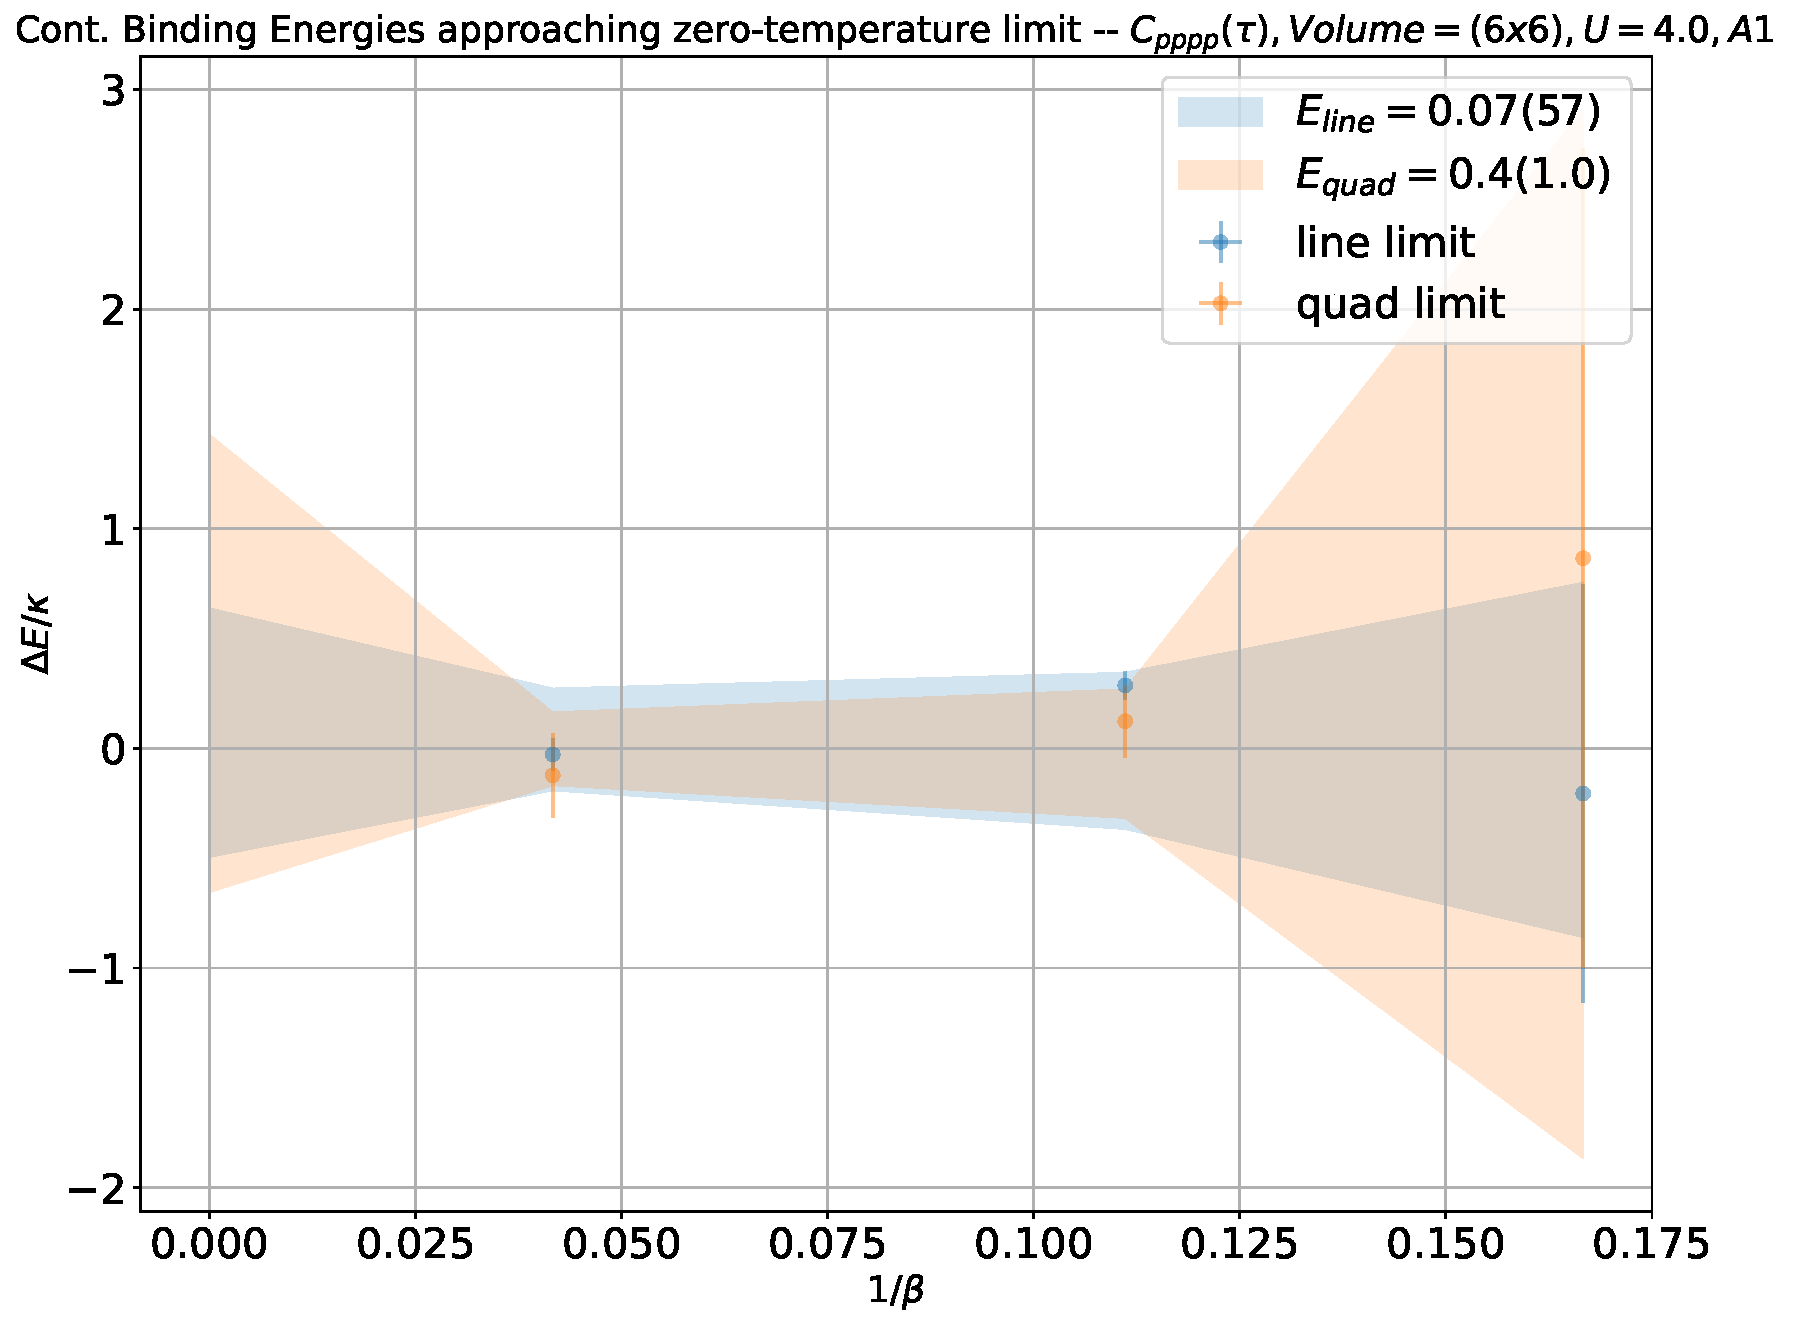
\includegraphics[width=\linewidth]{pppp-0-A1_6x6_U4.0_B24.0_temp.pdf}
    \end{subfigure}
    \begin{subfigure}{.5\textwidth}
        \centering
        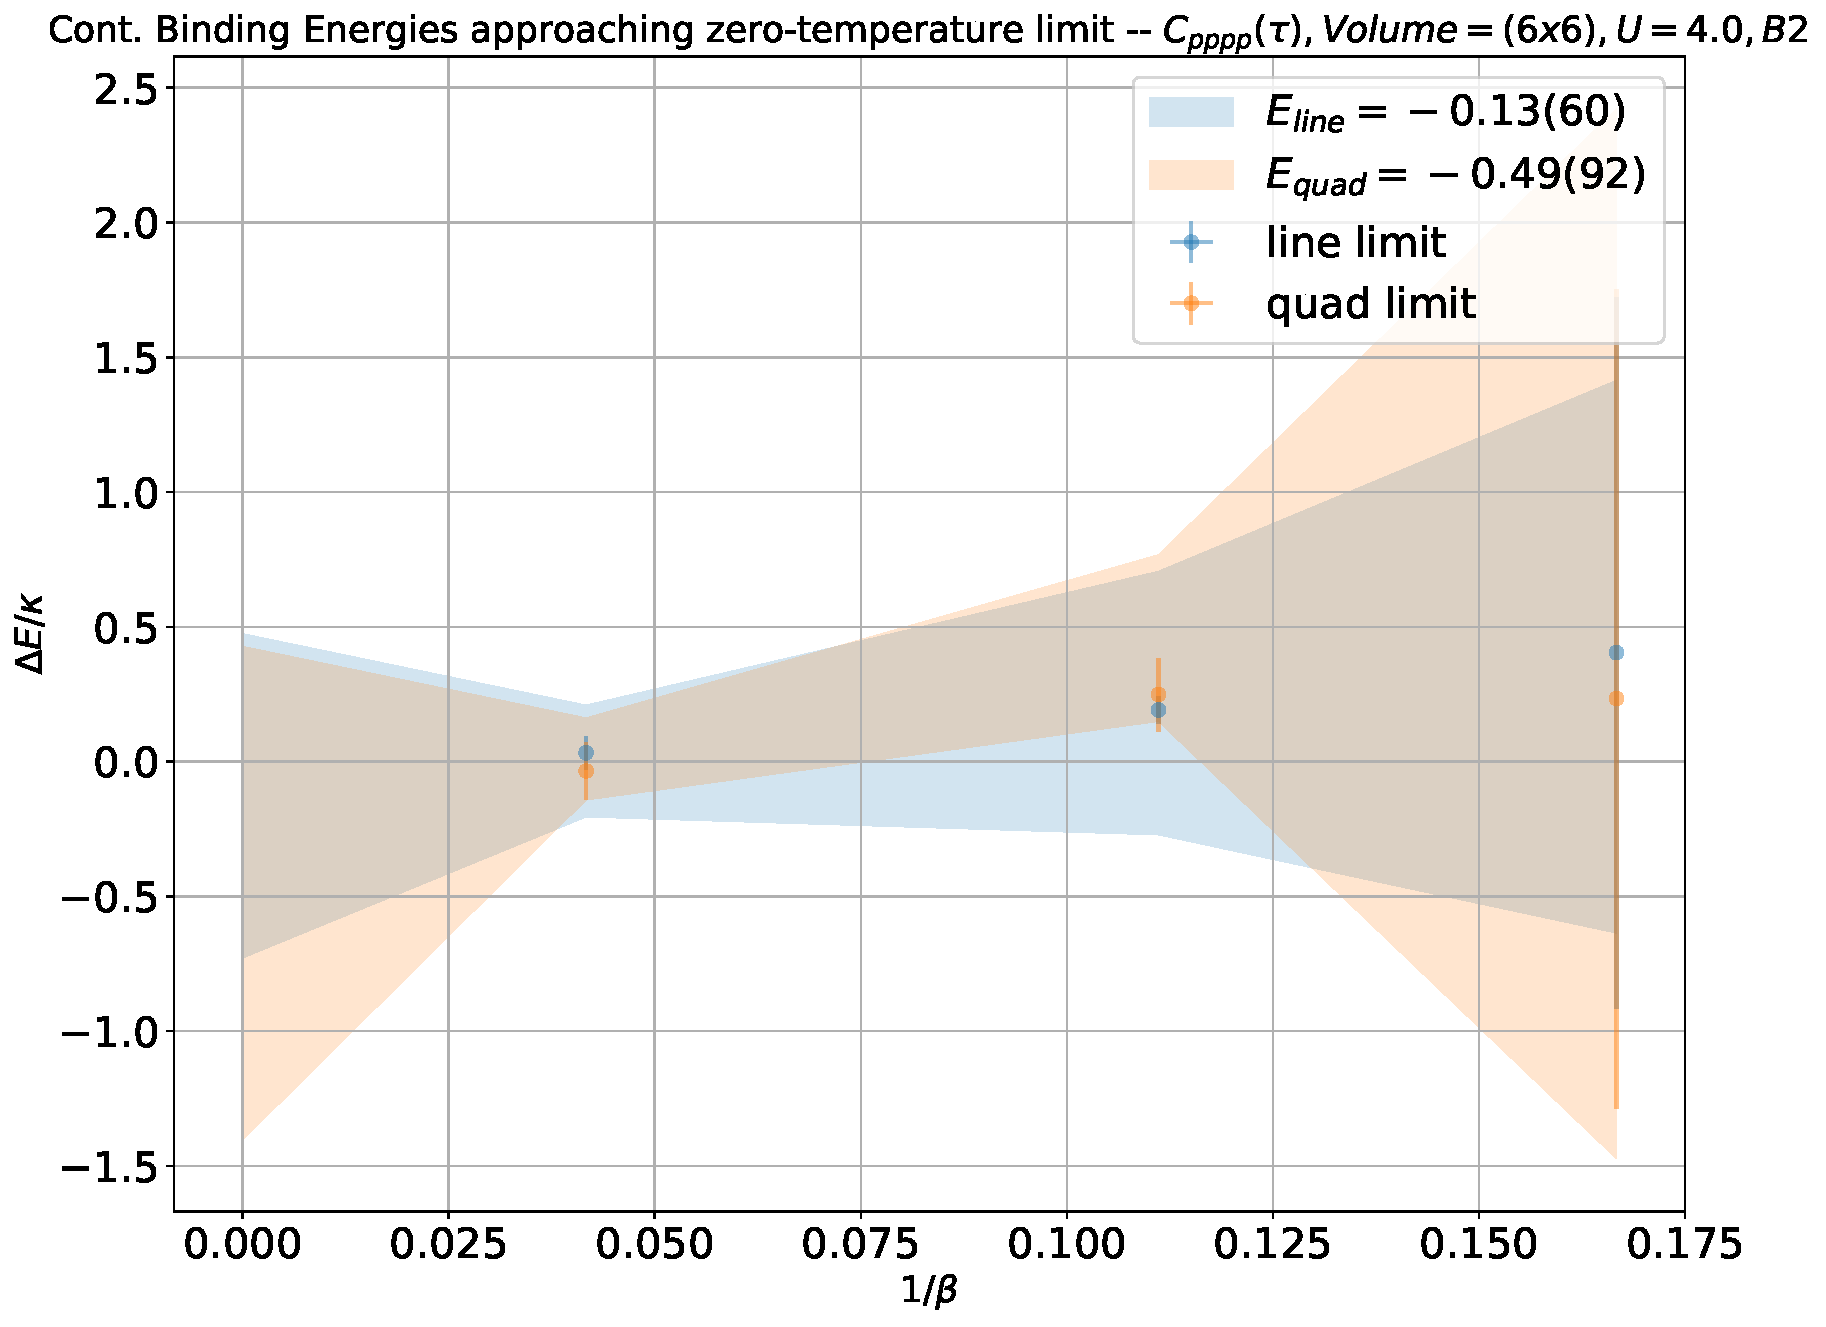
\includegraphics[width=\linewidth]{pppp-0-B2_6x6_U4.0_B24.0_temp.pdf}
    \end{subfigure}
    \caption{Zero-temperature extrapolation of continuum limit binding energies for $C_{phhp}$ and $C_{pppp}$ and both irreducible representations. This is done at lattice size $(6\times 6)$ and $U=4.0$. We plot it as a function of $1/\beta$ because it is simpler to show where the limit lies.}
    \label{fig:u4temp}
  \end{figure}
When above the critical coupling (\cref{fig:u4temp}) and there is a band gap, the binding energy of the particle-hole pair is clearly negative for $A1$ which is the symmetric state. However, $B2$ does not show the same behavior. It is a lot closer to zero, and we cannot conclusively tell whether there is a bound state. The particle-particle pair shows similar results for both couplings strengths that we measured. This correlator has the same behavior again for its irreducible representations and the binding energies are close to zero. Ensembles with the most probability for finding excitonic bound states are whenever there is a band gap, and we should be looking at operators transforming with $A1$ irreducible representations.

% If the results from both methods are equivalent up to the statistical uncertainties, we can be confident of our findings. There may be some interesting physics happening that will need further investigation. If the energies are different up to statistical error (that is, what we would expect), this may be due to the fact that the data obtained from the simulations or the model itself have strong intrinsic correlation that are not accounted in the first method.

% The fit of the data is done with a general cosine hyperbolic function. This is because we have symmetrized the functions. Working with the data shown in \cref{tab:work_ensembles}, we fit each lattice size independently, as we first need to reach the continuum limit for each lattice configuration and then extrapolate to the infinite volume limit. Results are performed. The results are done only for a total momentum $\Gamma$ and particle momenta $K,K'$.

% We calculate the binding energy (\cref{eq:binding_energy}) of the exciton by first extracting the energy from the two-body correlation function, then the energies of the one-body correlators. After a subtraction, we get $\epsilon$. 

% The next figures show the fitting of the correlators. As our data is symmetrized, we can fit a general cosine hyperbolic function instead of an exponential function. (PRE-REPHRASED)
